% !Mode:: "TeX:UTF-8"
%% 请使用 XeLaTeX 编译本文.
% \documentclass{WHUBachelor}% 选项 forprint: 交付打印时添加, 避免彩色链接字迹打印偏淡. 即使用下一行:
 \documentclass[forprint]{WHUBachelor}
\usepackage{amsmath, amsfonts, amssymb} % math equations, symbols
\usepackage[english]{babel}
\usepackage{color}      % color content
\usepackage{graphicx}   % import figures
\usepackage{url}        % hyperlinks
\usepackage{bm}         % bold type for equations
\usepackage{multirow}
\usepackage{booktabs}
\usepackage{epstopdf}
\usepackage{epsfig}
\usepackage{algorithm}
\usepackage{algorithmic}
\usepackage{esvect}
\usepackage{listings}
\usepackage[framed,numbered,autolinebreaks,useliterate]{mcode}
\usepackage{subfig}
\usepackage{float}
\usepackage{bm}
%\usepackage[unicode=true,pdfusetitle,bookmarks=true,bookmarksnumbered=false,bookmarksopen=false,breaklinks=false,pdfborder={0 0 1},backref=false,colorlinks=false]{hyperref}
%\usepackage[super,square,comma,sort&compress]{natbib}

\begin{document}
%%%%%%% 下面的内容, 据实填空.
\StudentNumber{2016011560} % 填写自己的学号

\title{\\Foundation of Finite Elements Method\\Assignment FEM model}

\author{易泽吉}                            % 作者名字

\Cmajor{工程力学}                  % 专业中文名

\Cschoolname{航天航空学院}          % 学院名

\date{二〇一八年三月}                    % 日期, 要注意和英文日期一致!!


%-----------------------------------------------------------------------------
\pdfbookmark[0]{封面}{title}         % 封面页加到 pdf 书签
\maketitle
\frontmatter
\pagenumbering{Roman}              % 正文之前的页码用大写罗马字母编号.
%-----------------------------------------------------------------------------

%==========================把目录加入到书签==============================%%%%%%
\pdfbookmark[0]{目录}{toc}
\mainmatter %% 以下是正文
%%%%%%%%%%%%%%%%%%%%%%%%%%%--------main matter-------%%%%%%%%%%%%%%%%%%%%%%%%%%%%%%%%%%%%

\section {3T单元}
\subsection {3T单元的建立}
3T单元是一种平面三角形线性单元,包括3个节点,每个节点有2个平面运动自由度。单元刚度阵规模为6×6。3T单元插值函数采用一次函数:
$ N_{1}^{e}=\frac{1}{2 A^{e}}\left[\left(x_{2}^{e} y_{3}^{e}-x_{3}^{e} y_{2}^{e}\right)+y_{23}^{e} x+x_{32}^{e} y\right] $
$ N_{2}^{e}=\frac{1}{2 A^{e}}\left[\left(x_{3}^{e} y_{1}^{e}-x_{1}^{e} y_{3}^{e}\right)+y_{31}^{e} x+x_{13}^{e} y\right] $
$ N_{3}^{e}=\frac{1}{2 A^{e}}\left[\left(x_{1}^{e} y_{2}^{e}-x_{2}^{e} y_{1}^{e}\right)+y_{12}^{e} x+x_{21}^{e} y\right] $

\begin{figure}[H]
\centering  
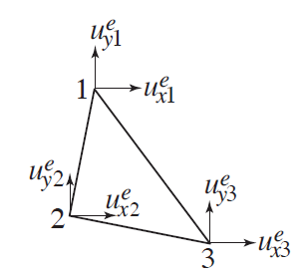
\includegraphics[width = .4\textwidth]{t3_1.png} 
\caption{3T单元示意图} 
\label{f1.1} 
\end{figure}

该插值函数满足归一化条件,包含$ 1、x、y $项,能够准确插值线性场。且由于形函数线性,应变矩阵$ B^{e} $为常数,即3T单元为常应变单元。3T单元刚度阵计算如下:
$ \boldsymbol{B}^{e}=\frac{1}{2 A^{e}}\left[\begin{array}{cccccc}{y_{23}^{e}} & {0} & {y_{31}^{e}} & {0} & {y_{12}^{e}} & {0} \\ {0} & {x_{32}^{e}} & {0} & {x_{13}^{e}} & {0} & {x_{21}^{e}} \\ {x_{32}^{e}} & {y_{23}^{e}} & {x_{13}^{e}} & {y_{31}^{e}} & {x_{21}^{e}} & {y_{12}^{e}}\end{array}\right] $
$ \boldsymbol{K}^{e}=\int_{\Omega^{e}} \boldsymbol{B}^{e \mathrm{T}} \boldsymbol{D} \boldsymbol{B}^{e} \mathrm{d} \Omega=t^{e} A^{e} \boldsymbol{B}^{e \mathrm{T}} \boldsymbol{D} \boldsymbol{B}^{e} $

单元应变计算如下:
$ \boldsymbol{\varepsilon}^{e}=\nabla_{S} \boldsymbol{u}^{e}=\boldsymbol{B}^{e} \boldsymbol{d}^{e} $
结果确为常应变。

\subsection {3T单元的Patch Test}
选取一个6节点6单元的不规则网格划分如\ref{f2},构造一个单轴拉伸的线性场,进行Patch Test C测试,选取参数$E=1×10^{7}$,$\nu=0.3$,$t=1$,$F=10$。

\begin{figure}[H]
\centering  
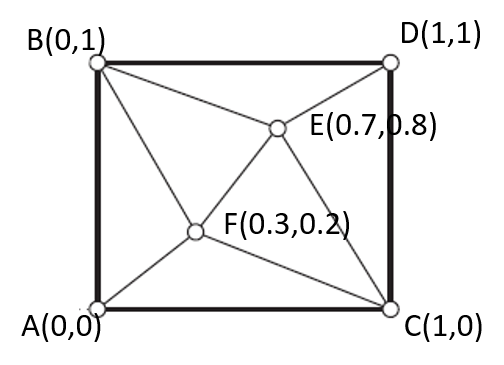
\includegraphics[width = .6\textwidth]{t3_2.png} 
\caption{Patch Test网格划分} 
\label{f1.2} 
\end{figure}

测试结果如下,在忽略极小的浮点误差下与单轴拉伸的理论结果完全一致。

\begin{figure}[H]
\centering  
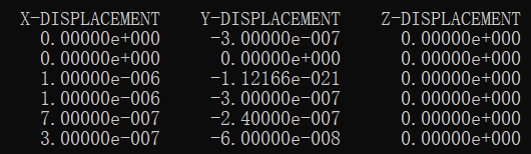
\includegraphics[width = .8\textwidth]{t3_3.png} 
\caption{Patch Test结果} 
\label{f1.3} 
\end{figure}

与建模时候的预测相同,3T单元能够准确复现线性场,达到预期的一阶收敛率。

\subsection {3T单元收敛率分析}
收敛率分析选取一个二次问题,一端固定的正方形薄板受均匀体力拉伸。网格划分时先将网格划分为长度为$h$的小的正方形网格,再沿45°方向将正方形划分成两个三角形。

\begin{figure}[H]
\centering  
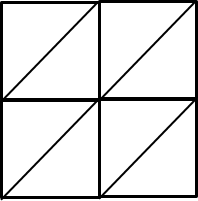
\includegraphics[width = .4\textwidth]{t3_4.png} 
\caption{收敛率分析网格示意图} 
\label{f1.4} 
\end{figure}

选择网格边长为正方形边长的1/2至1/6,分别计算各节点的位移,对节点位移进行插值得到有限元解的位移场。求有限元解与实际二次解的位移差的范数,做双对数图即可得到收敛率。结果为2,符合对线性场的估计。

\begin{figure}[H]
\centering  
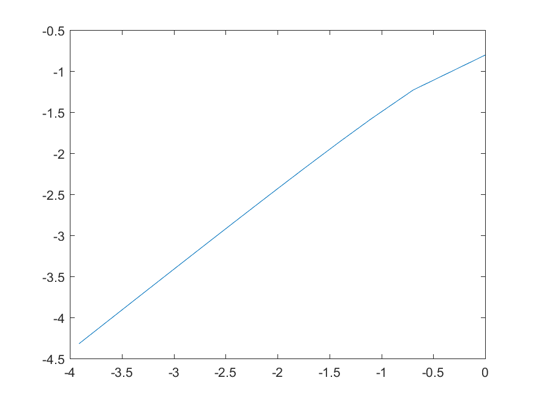
\includegraphics[width = .8\textwidth]{t3_5.png} 
\caption{收敛率双对数图} 
\label{f1.5} 
\end{figure}

\section{8H单元}
\subsection{8H单元的建立}
8H单元是一种三维拉压单元,8节点24自由度。插值时采用母单元插值方法,即构造一个母单元,建立母单元与实际单元之间的一一映射关系,通过在母单元插值后映射到实际单元完成对实际单元的插值。

\begin{figure}[H]
\centering  
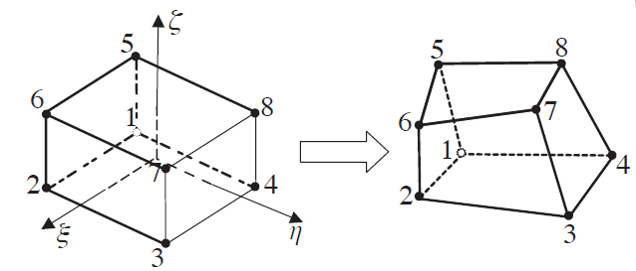
\includegraphics[width = .8\textwidth]{h8_1.png} 
\caption{8H单元d1母单元与实际单元} 
\label{f2.1} 
\end{figure}

母单元插值函数为三方向线性插值函数的积:
$\begin{aligned} N_{L}^{8 \mathrm{H}}(\xi, \eta, \zeta) &=N_{I}^{2 L}(\xi) N_{J}^{2 L}(\eta) N_{K}^{2 L}(\zeta) \\ &=\frac{1}{8}\left(1+\xi_{L} \xi\right)\left(1+\eta_{L} \eta\right)\left(1+\zeta_{L} \zeta\right) \end{aligned}$
坐标映射Jacobian矩阵为:
$ \ensuremath{\begin{aligned}J^{e} & =GN^{8H}\left[x^{e}y^{e}\right]\\
 & =\ensuremath{\left[\begin{array}{cccc}
\frac{\partial N_{1}^{8\mathrm{H}}}{\partial\xi} & \frac{\partial N_{2}^{8\mathrm{H}}}{\partial\xi} & \cdots & \frac{\partial N_{8}^{8\mathrm{H}}}{\partial\xi}\\
\frac{\partial N_{1}^{8\mathrm{H}}}{\partial\eta} & \frac{\partial N_{2}^{8\mathrm{H}}}{\partial\eta} & \cdots & \frac{\partial N_{8}^{8\mathrm{H}}}{\partial\eta}\\
\frac{\partial N_{1}^{8\mathrm{H}}}{\partial\zeta} & \frac{\partial N_{2}^{8\mathrm{H}}}{\partial\zeta} & \cdots & \frac{\partial N_{8}^{8\mathrm{H}}}{\partial\zeta}
\end{array}\right]\left[\begin{array}{cc}
x_{1}^{e} & y_{1}^{e}\\
x_{2}^{e} & y_{2}^{e}\\
\vdots & \vdots\\
x_{8}^{e} & y_{8}^{e}
\end{array}\right]}
\end{aligned}
} $
应变矩阵$B^{e}$满足:
$ B^{e}=\left[\begin{array}{cccc}$
$B_{1}^{e} & B_{2}^{e} & \cdots & B_{8}^{e}\end{array}\right]$
 

其中:$B_{i}^{e}=\left[\begin{array}{ccc}
\frac{\partial N_{i}^{8\mathrm{H}}}{\partial x} & 0 & 0\\
0 & \frac{\partial N_{i}^{8\mathrm{H}}}{\partial y} & 0\\
0 & 0 & \frac{\partial N_{i}^{8\mathrm{H}}}{\partial z}\\
0 & \frac{\partial N_{i}^{8\mathrm{H}}}{\partial z} & \frac{\partial N_{i}^{8\mathrm{H}}}{\partial y}\\
\frac{\partial N_{i}^{8\mathrm{H}}}{\partial z} & 0 & \frac{\partial N_{i}^{8\mathrm{H}}}{\partial x}\\
\frac{\partial N_{i}^{8\mathrm{H}}}{\partial y} & \frac{\partial N_{i}^{8\mathrm{H}}}{\partial x} & 0
\end{array}\right](i=1,2,\cdots,8)$
 
$B^{e}$的元素满足:
$\left[\begin{array}{cccc}
\frac{\partial N_{1}^{8\mathrm{H}}}{\partial x} & \frac{\partial N_{2}^{8\mathrm{H}}}{\partial x} & \cdots & \frac{\partial N_{8}^{8\mathrm{H}}}{\partial x}\\
\frac{\partial N_{1}^{8\mathrm{H}}}{\partial y} & \frac{\partial N_{2}^{8\mathrm{H}}}{\partial y} & \cdots & \frac{\partial N_{8}^{8\mathrm{H}}}{\partial y}\\
\frac{\partial N_{1}^{8\mathrm{H}}}{\partial z} & \frac{\partial N_{2}^{8\mathrm{H}}}{\partial z} & \cdots & \frac{\partial N_{8}^{8\mathrm{H}}}{\partial z}
\end{array}\right]=(J^{e})^{-1}GN^{8\mathrm{H}}$

 $B^{e}$不是常系数矩阵,单元刚度阵$K^{e}$需要积分获得。假设$J^{e}$的行列式为常数,则被积函数为2次,需要2×2×2的高斯积分。实际编程时分别直接计算8个高斯点对应的$J^{e}$、$B^{e}$和被积函数的值,再加权相加即可得到单元刚度阵。

\subsection{8H单元的Patch Test}
 由于一一映射的要求,8H单元必须是凸六面体单元,故选择一个大立方体套小立方体的结构,共16节点7单元。其中大立方体边长为1,小立方体与大立方体平行且中心重合,边长为0.6。加载形式为无重力单轴拉伸,参数$E=1×10^{7}$,$\nu=0.3$,$t=1$,$F=100$。            

\begin{figure}[H]
\centering  
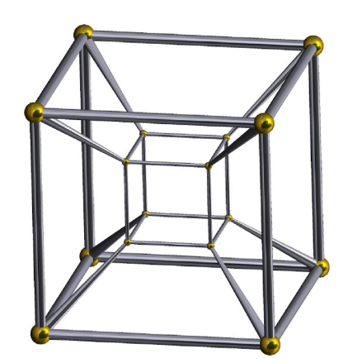
\includegraphics[width = .4\textwidth]{h8_2.png} 
\caption{Patch Test网格划分} 
\label{f2.2} 
\end{figure}

结果如下。8H单元能够在浮点精度下通过线性分片实验,说明该单元收敛。

\begin{figure}[H]
\centering  
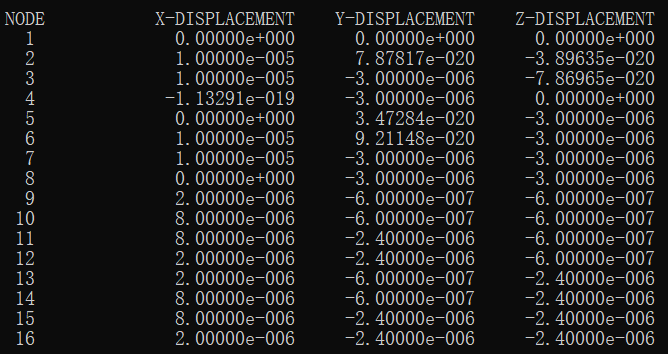
\includegraphics[width = .8\textwidth]{h8_3.png} 
\caption{Patch Test结果} 
\label{f2.3} 
\end{figure}

\subsection{8H单元的收敛率}
选择一个一端固定,受均匀体力拉伸的块体为对象进行收敛率分析。网格划分为等大的立方体,边长取1/2~1/6。将有限元位移场与理论值比较,作误差的双对数图线如下。
\begin{figure}[H]
\centering  
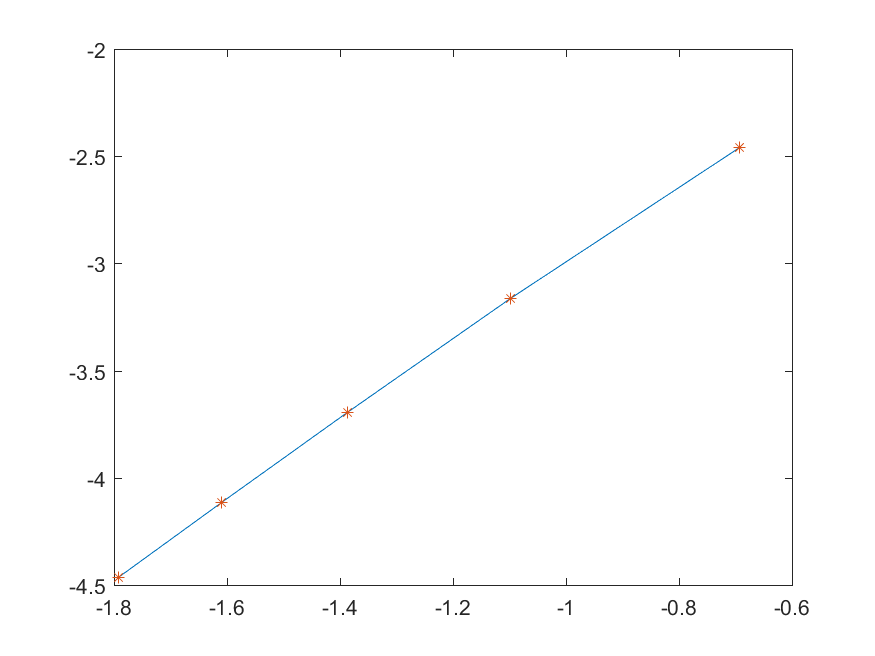
\includegraphics[width = .8\textwidth]{h8_4.png} 
\caption{收敛率双对数图} 
\label{f2.4} 
\end{figure}

可以看出,收敛率为2,符合一般线性单元的特征。
\section{前处理}
前处理采用python实现,数据存储时采用了python自带的顺序链表和字典,没有用任何库文件,版本为3.7。文件需要读取的主要信息包括part内部的单元,结点,材料信息,part 通过先平移后旋转后得到的instance信息,边界条件与不同instance之间的连接信息。已经实现的前处理程序大约1500行,能够顺利实现4个算例以及我们自己画的桥的inp文件读取,耗时均在10s以内,当遇到了新的单元,单元内部新的关键字名称,连接的两个点坐标差距在浮点数误差以上时均有报错语句,而且有能够实现不同位置结点连接时寻找最合适的连接点的算法。此外,还用matlab做了可视化,从图片中可以清楚的看出桥的约束以及各单元位置,在进一步的验证正确性环节,在整体stap++程序无法运行时可以对第一个文件手动找出所有连接点连接情况和对应坐标,对已经成功运行后可以把后处理中夸张系数调大100倍后判断是否有未连接上的点对,计算最终点数目判断是否有多连接的点对(如第一个文件应当最后点的数目为4091)。用这种方法我们成功发现了我们自己设计的桥在abaqus设计时连接错了的点对,并在前处理程序中成功调整(事实上即使你把连接点中的一个往上移数个单元abaqus也能给出结果,但显然会带来一定误差。下面是matlab可视化图片
\begin{figure}[H]
\centering  
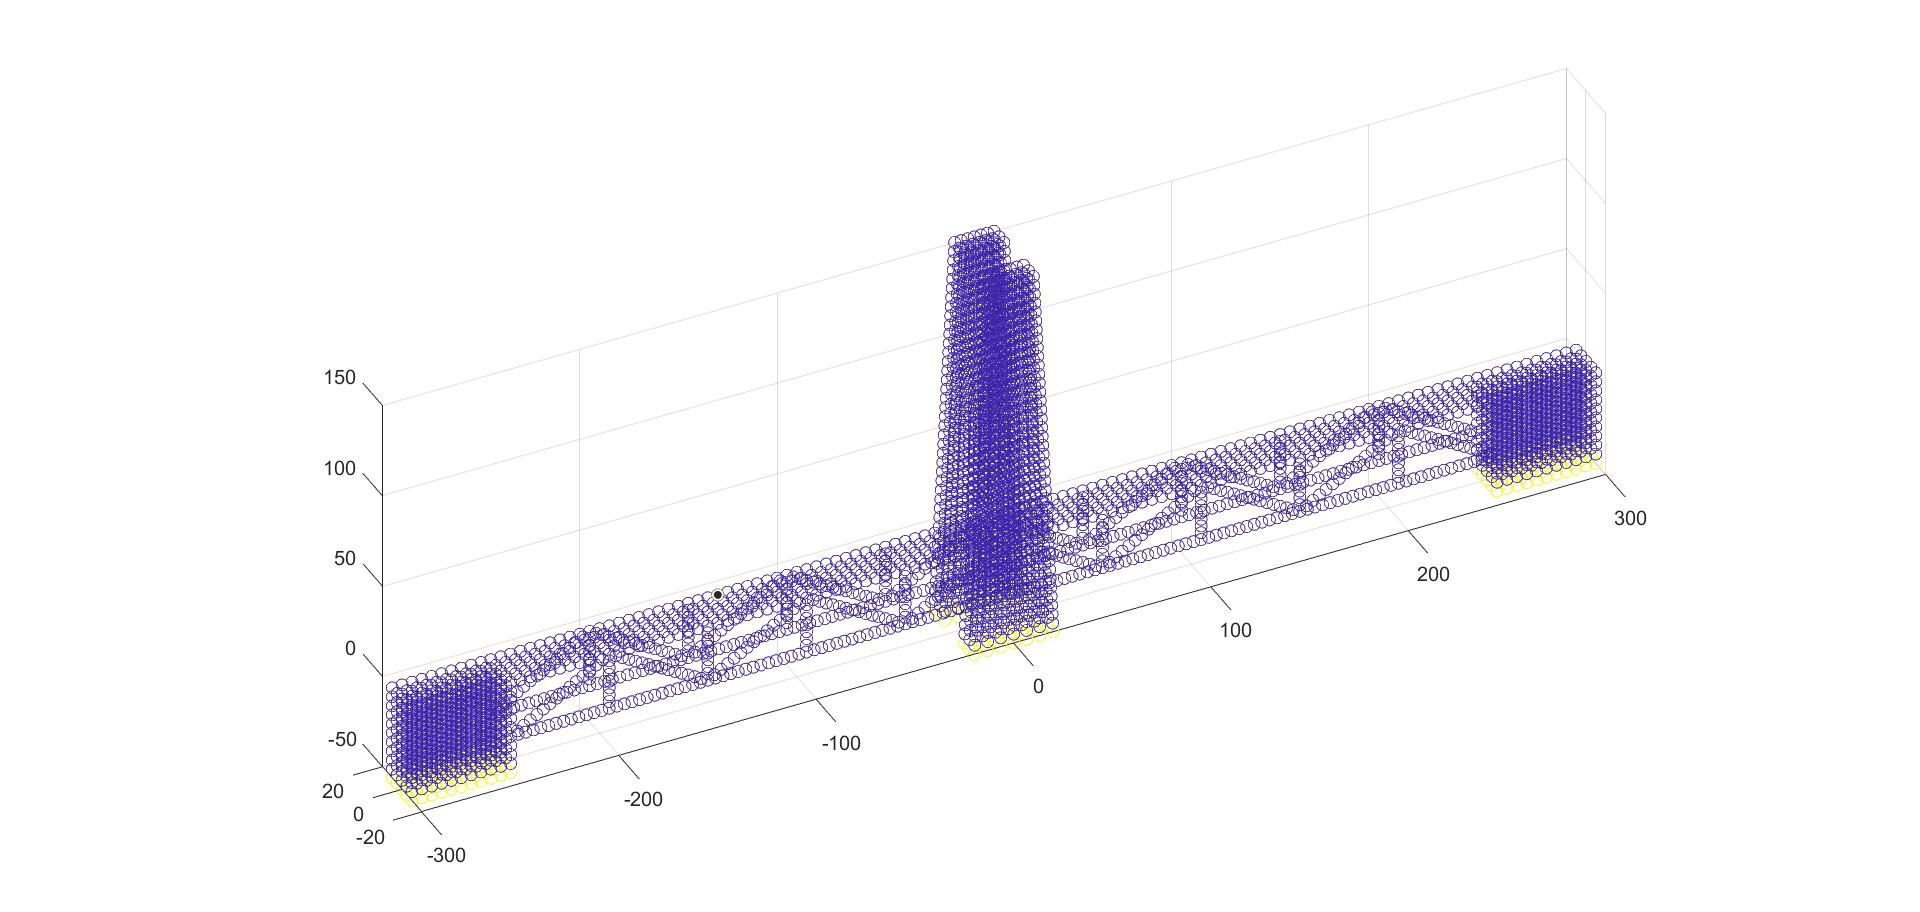
\includegraphics[width = .8\textwidth]{boundary_1.jpg} 
\caption{第一座桥的边界条件图} 
\label{f3.1} 
\end{figure}
\begin{figure}[H]
\centering  
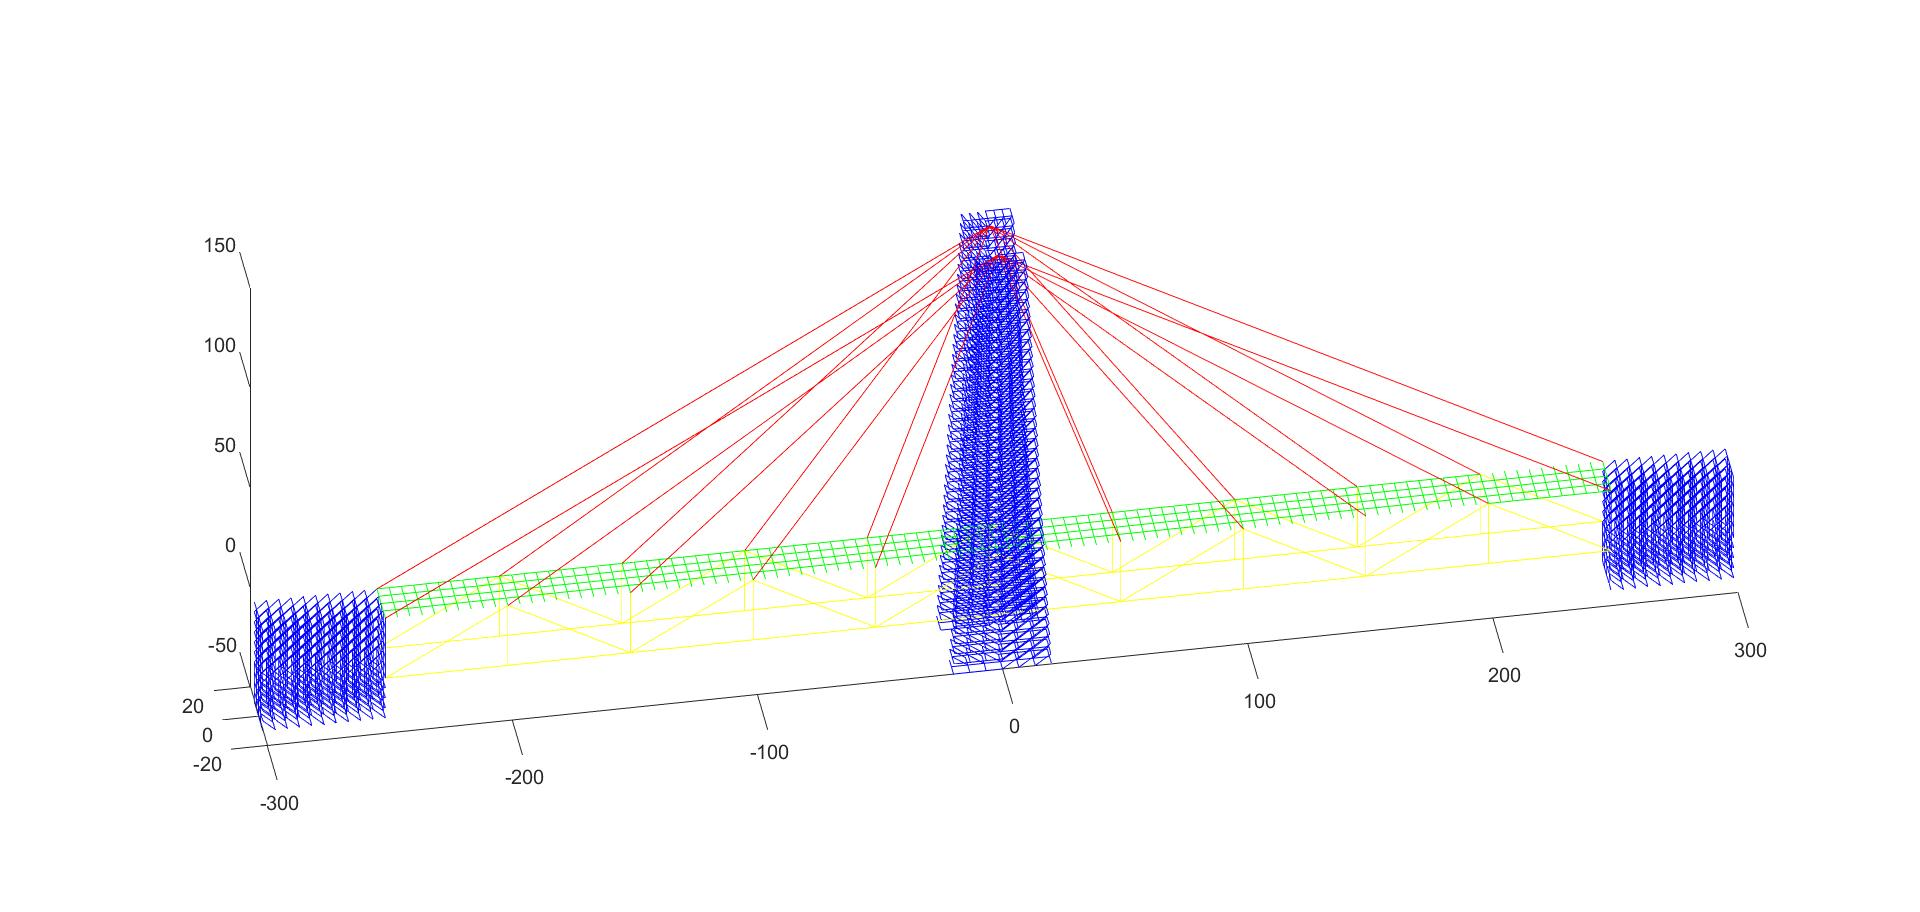
\includegraphics[width = .8\textwidth]{element_1.jpg} 
\caption{第一座桥单元图} 
\label{f3.2} 
\end{figure}
\begin{figure}[H]
\centering  
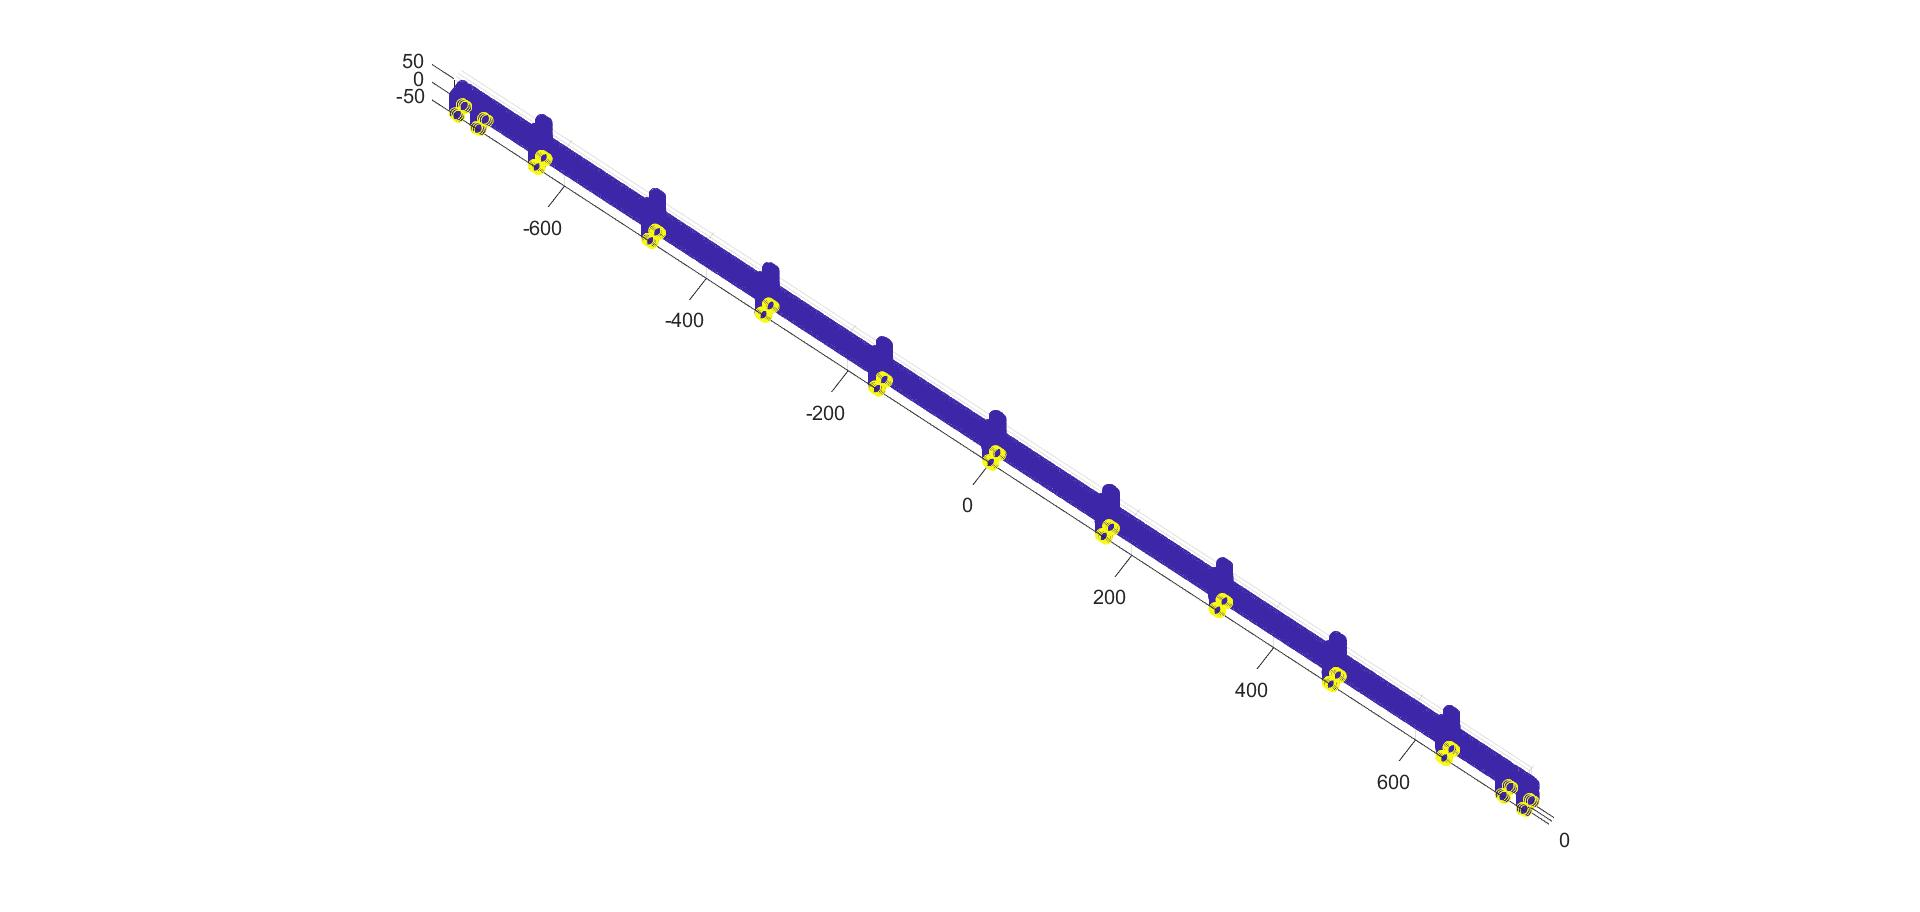
\includegraphics[width = .8\textwidth]{boundary_2.jpg} 
\caption{我们自己设计的桥的边界条件图} 
\label{f3.3} 
\end{figure}

\section{后处理}
后处理采用vtk格式实现。某次实验输出的vtk格式结果样图如下。vtk信息中包含各节点、单元的几何信息,六个方向的位移和Mises应力。stap++每次执行输出两个vtk文件,分别对应变形前和变形后的几何信息,七个物理量的信息完全一致。
\begin{figure}[H]
\centering  
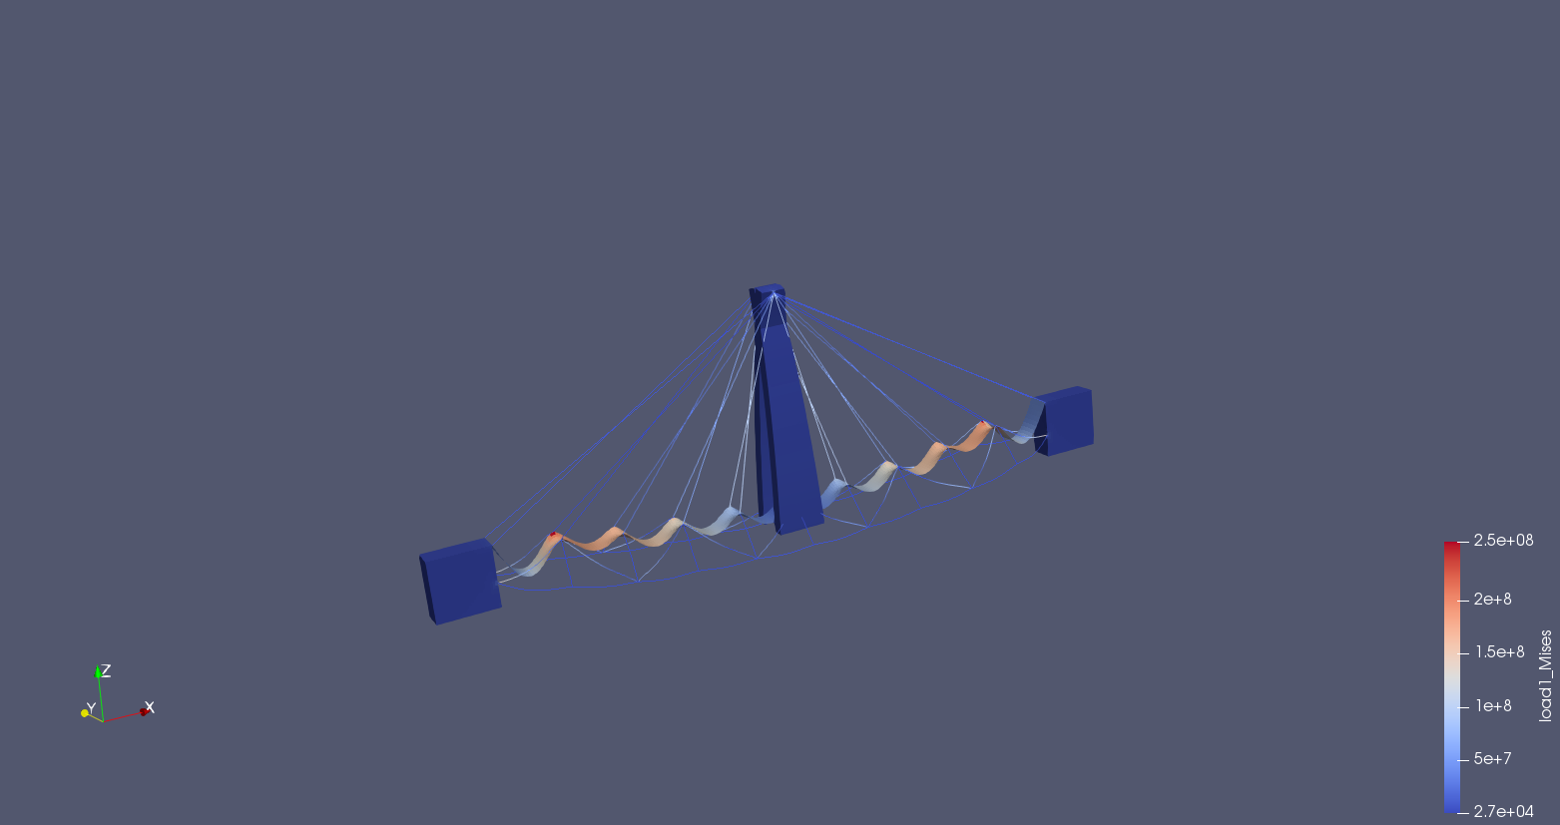
\includegraphics[width = .8\textwidth]{vtk_1.png} 
\caption{输出结果样图} 
\label{f3.1} 
\end{figure}
本次实验使用的vtk文件包括控制行、节点信息、单元信息、节点物理量、单元物理量四个部分。典型的vtk的部分图如下:
\begin{figure}[H]
\centering  
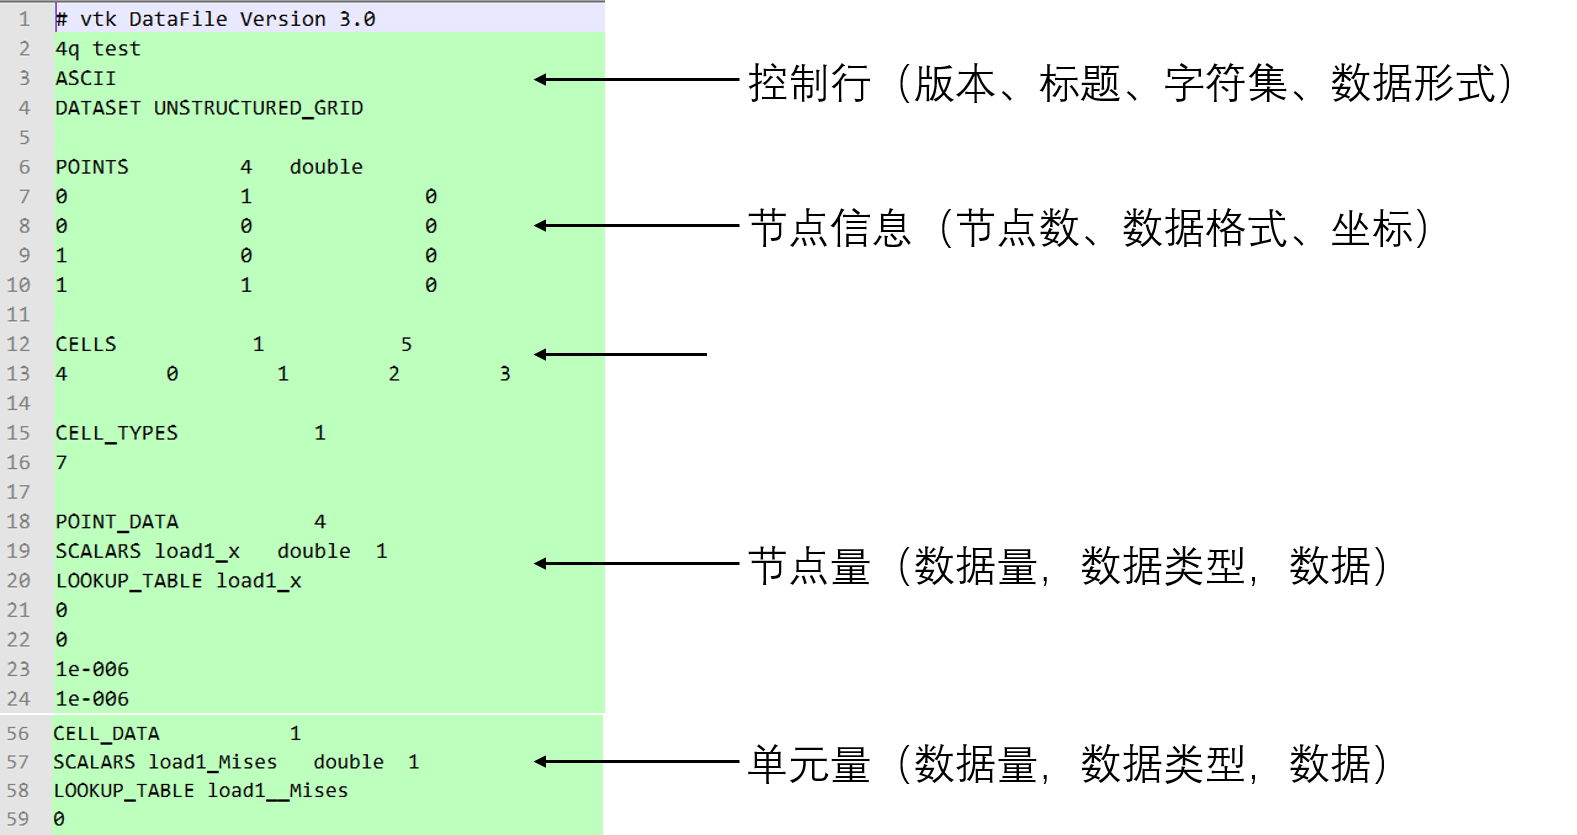
\includegraphics[width = .8\textwidth]{vtk_2.png} 
\caption{一个典型的vtk文件(部分)} 
\label{f3.2} 
\end{figure}
其中控制行在程序开始执行时输出。变形前的节点和单元信息分别在读取节点和单元信息之后立即输出,保证即使无法求解也能够绘制出几何信息,便于查错。当位移计算完成时,在变形前的vtk中写入六个方向的位移信息;在变形后的vtk中先按照原始位形与位移和夸张系数计算出新的节点坐标,再依次输出单元信息和位移信息。当在向.out结果文件中写入应力后,依次向两个vtk中写入应力信息。为方便起见,每个单元写入的Mises应力为单元全部高斯点的Mises应力的平均值。

\section{板单元(Plate Element)}

\subsection{板单元的基本公式}

我们选用的板单元为4节点Kirchoff板单元,如图\ref{f1}所示:

\begin{figure}[H]
\centering  
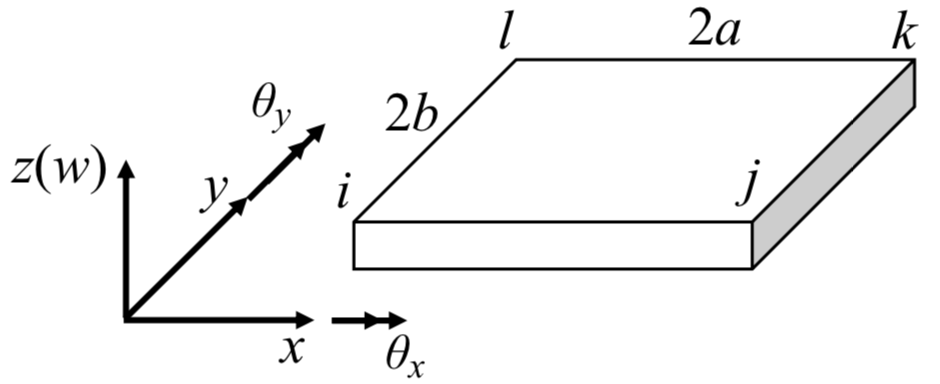
\includegraphics[width = .5\textwidth]{1.png} 
\caption{Kirchoff板单元结构示意图} 
\label{f1} 
\end{figure}

其中每一个节点具有一个垂直于板的位移自由度$w$和绕板平面内两个垂直轴,即$x$轴和$y$轴的转角$\text{\ensuremath{\theta_{x}},\ensuremath{\theta_{y}}}$,同时Kirchoff板遵循平截面和直法线假设,因此板内部的位移场为:

\begin{equation}
\begin{array}{l}
{u=u_{0}+z\theta_{y}}\\
{v=v_{0}-z\theta_{x}}\\
{w=w_{0}(x,y)}
\end{array}\label{eq1}
\end{equation}

其中转角和挠度的关系为:

\begin{equation}
\theta_{x}=\frac{\partial w}{\partial y},\quad\theta_{y}=-\frac{\partial w}{\partial x}\qquad\gamma_{xz}=\gamma_{yz}=0\label{eq2}
\end{equation}

代入到应变和转角的关系中可以得到:

\begin{equation}
\boldsymbol{\varepsilon}=\left\{ \begin{array}{c}
{\varepsilon_{x}}\\
{\varepsilon_{y}}\\
{\gamma_{xy}}
\end{array}\right\} =z\left\{ \begin{array}{c}
{-\frac{\partial^{2}w}{\partial x^{2}}}\\
{-\frac{\partial^{2}w}{\partial y^{2}}}\\
{-2\frac{\partial^{2}w}{\partial x\partial y}}
\end{array}\right\} \label{eq3}
\end{equation}

可见在此假设下板单元的应力场只有三个分量

\subsection{板单元的应力应变以及刚度阵构造}

由公式(\ref{eq3})再代入应力应变关系中可以得到:

\begin{equation}
\left[\begin{array}{c}
{\sigma_{x}}\\
{\sigma_{y}}\\
{\tau_{xy}}
\end{array}\right]=\frac{E}{1-v^{2}}\left[\begin{array}{ccc}
{1} & {v} & {0}\\
{v} & {1} & {0}\\
{0} & {0} & {\frac{1-v}{2}}
\end{array}\right]\left[\begin{array}{c}
{\varepsilon_{x}}\\
{\varepsilon_{y}}\\
{\gamma_{xy}}
\end{array}\right]\label{eq4}
\end{equation}

由于三个应力分量和坐标$z$呈现线性关系,因此进行积分得到相应的力矩:

\begin{equation}
\begin{aligned}M & =\left\{ \begin{array}{l}
{M_{x}}\\
{M_{y}}\\
{M_{xy}}
\end{array}\right\} =\boldsymbol{D}\boldsymbol{\kappa}=\boldsymbol{D}\boldsymbol{L}w\\
M_{x} & =\int_{-t/2}^{t/2}z\sigma_{x}\mathrm{d}z\\
M_{y} & =\int_{-t/2}^{t/2}z\sigma_{y}\mathrm{d}z\\
M_{xy} & =\int_{-t/2}^{t/2}z\tau_{xy}\mathrm{d}z
\end{aligned}
\label{eq5}
\end{equation}

而最终的方程:

\begin{equation}
\boldsymbol{L}^{\mathrm{T}}\boldsymbol{D}\boldsymbol{L}w-q=0\label{eq6}
\end{equation}

最后构造w的差值函数(由于每一个板单元有12个自由度,因此构造一个具有12项的三次完备多项式):

\begin{equation}
w^{e}=\bm{P}\bm{\alpha^{e}}\label{eq7}
\end{equation}
然后利用节点的位移以及转角得到:

\begin{equation}
\bm{d^{e}}=\bm{M}\bm{\alpha}^{e}\label{eq8}
\end{equation}
代入公式(\ref{eq7})可以得到:

\begin{equation}
\begin{array}{c}
w^{e}=\bm{Nd^{e}}\\
\bm{N=PM^{-1}}
\end{array}\label{eq9}
\end{equation}
进行简单的坐标变换可以得到矩形板单元的形函数表达式:

\begin{equation}
\text{\ensuremath{\bm{N^{T}}=\frac{1}{8}\begin{bmatrix}-(s-1)(t-1)(s^{2}+s+t^{2}+t-2)\\
-b(s-1)(t-1)^{2}(t+1)\\
a(s-1)^{2}(s+1)(t-1)\\
(s+1)(t-1)(s^{2}-s+t^{2}+t-2)\\
b(s+1)(t-1)^{2}(t+1)\\
a(s+1)^{2}(s-1)(t-1)\\
-(s+1)(t+1)(s^{2}-s+t^{2}-t-2)\\
b(s+1)(t+1)^{2}(t-1)\\
-a(s+1)^{2}(s-1)(t+1)\\
(s-1)(t+1)(s^{2}+s+t^{2}-t-2)\\
-b(s-1)(t+1)^{2}(t-1)\\
-a(s-1)^{2}(s+1)(t+1)
\end{bmatrix}}}\label{eq10}
\end{equation}
对形函数$\bm{N}$进行求导得到:

\begin{equation}
\bm{B}=\bm{LN}\label{eq11}
\end{equation}
相应的力矩$\text{\ensuremath{\bm{M}=\bm{DBd^{e}}}}$,从而我们得到单元刚度阵(单元的长,宽分别为$2a,2b$):

\begin{equation}
\bm{K}=ab\int_{-1}^{1}\int_{-1}^{1}\bm{B^{T}DB}{\rm d}s{\rm d}t\label{eq12}
\end{equation}
将公式(\ref{eq10})和公式(\ref{eq11})代入(\ref{eq12})中,并用matlab进行符号运算得到刚度阵的元素,然后利用skyline的存储方式输入到Stap++的Plate类的单元Stiffmatrix函数中

\subsection{应力计算以及后处理}

将单元刚度阵组装之后计算得到整体刚度阵中板单元的贡献;于此同时,对受力进行等效到节点上:

\begin{equation}
f_{i}=\left\{ \begin{array}{l}
{f_{w_{i}}}\\
{f_{\theta_{i_{i}}}}\\
{f_{\theta_{i_{i}}}}
\end{array}\right\} =\int_{-b}^{b}\int_{-a}^{a}N^{\mathrm{T}}q\mathrm{d}x\mathrm{d}y\label{eq13}
\end{equation}
对于重力的作用:$q=\rho gt$($t$为板单元的厚度,$\rho$为材料密度,$g$为重力加速度),代入公式(\ref{eq13})可以得到:

\begin{equation}
\begin{array}{l}
{f_{1z}=-\frac{1}{12}\rho gtab\left\{ \begin{array}{c}
{3}\\
{b}\\
{-a}
\end{array}\right\} \quad f_{2}=-\frac{1}{12}\rho gtab\left\{ \begin{array}{c}
{3}\\
{-b}\\
{-a}
\end{array}\right\} }\\
{f_{3}=-\frac{1}{12}\rho gtab\left\{ \begin{array}{l}
{3}\\
{b}\\
{a}
\end{array}\right\} \quad f_{4}=-\frac{1}{12}\rho gtab\left\{ \begin{array}{c}
{3}\\
{-b}\\
{a}
\end{array}\right\} }
\end{array}\label{eq14}
\end{equation}
同样将其组装到整体的方程中,可以求解相应的节点位移和转角。

利用求解得到的位移和转角代入公式(\ref{eq9})中可以得到相应的挠度分布,仅以不由转角-挠度关系(\ref{eq2})可以得到单元内部的转角分布

关于应力,由(\ref{eq3})可知:应力和应变在中性面的值为0,在表面最大,因此我们可以选择输出表面的应力$(z=\pm\frac{t}{2})$或者$z$方向高斯点$(z=\pm\frac{t}{2\sqrt{3}})$的应力:

\begin{equation}
\begin{array}{cc}
\text{表\text{面}} & \bm{\sigma_{(\pm)}^{e}=}\pm\frac{6}{t^{2}}\bm{M^{e}}\\
Gauss\text{点} & \bm{\sigma_{(\pm)}^{e}=}\pm\frac{6}{\sqrt{3}t^{2}}\bm{M^{e}}
\end{array}\label{eq15}
\end{equation}
最后针对后处理的输出,可以输出相应上下表面对应xy平面的Gauss点的Mises应力,然后取其平均值作为该单元的Mises应力。

\subsection{输入文件格式和自由度约束}

主体的输入文件格式基本不变,但是对于板单元而言,其节点只有三个自由度,也就是说其另外三个自由度是锁死的,那么对于倾斜的板单元,其对应的约束就较为复杂,需要利用旋转刚度阵将其进行坐标变换,由于最终的桥梁算例中,板单元都是位于xy平面内的,因此在Stap++中并没有实现倾斜板的功能;在此情况下输入文件中6个bcode数中,前两个(bcode{[}0{]},bcode{[}1{]})和最后一个(bcode{[}5{]})都应该设为1,而其余几个bcode数则根据具体的模型约束情况而定,我们以一个板单元的输入文件为例子,如图\ref{f2}所示:

\begin{figure}[H]
\centering  
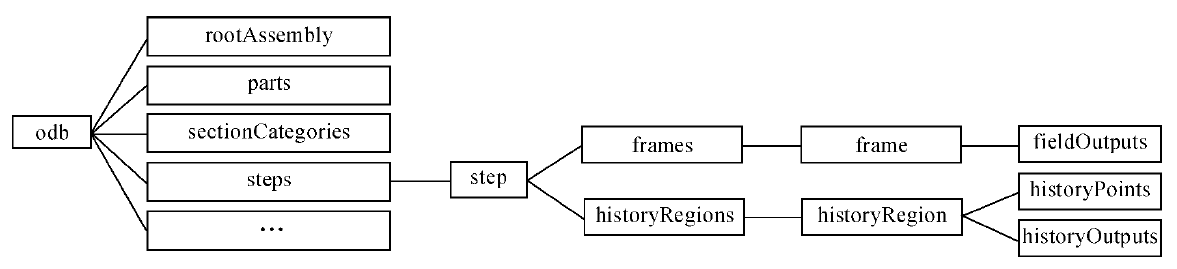
\includegraphics[width = .8\textwidth]{2.png} 
\caption{1个单元的板单元输入文件示意图} 
\label{f2} 
\end{figure}

而后续的节点力则按照公式(\ref{eq14})添加,格式和其他单元一致。

\subsection{分片测试}

我们在$[-1,1]^{2}$的正方形板构造这样的位移场 $w=x^{2}-\nu y^{2}$, 由公式(\ref{eq2})可以得到:

\begin{equation}
\begin{array}{c}
\theta_{x}=-2\nu y\\
\theta_{y}=-2x
\end{array}\label{eq16}
\end{equation}
由公式(\ref{eq5})可以得到均匀弯矩场:

\begin{equation}
\bm{M^{e}=}\begin{bmatrix}-\frac{1}{6}Et^{3}\\
0\\
0
\end{bmatrix}\label{eq17}
\end{equation}
其中$E=30,\nu=0.2,t=1$;利用$x=0$;$y=0$;$y=0.5$三条直线 将正方形板分割成六个分片,如图\ref{f3}所示:

\begin{figure}[H]
\centering  
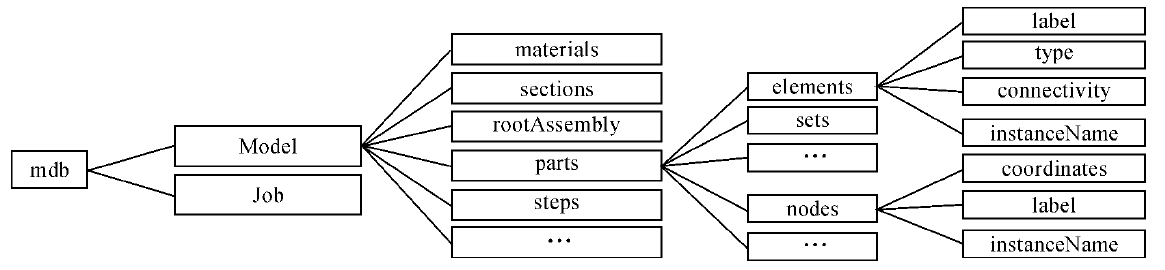
\includegraphics[width = .3\textwidth]{3.png} 
\caption{Plate单元分片实验划分示意图} 
\label{f3} 
\end{figure}

对应的将法线沿 x 轴方向边界($x=\pm1$)上的 y 向弯矩分配到边界上的每个点上:

\begin{equation}
\begin{array}{c}
M_{4y}=-M_{1y}=-2.5\\
M_{8y}=-M_{5y}=-5\\
M_{12y}=-M_{9y}=-2.5
\end{array}\label{eq18}
\end{equation}

具体输入文件见 Platepatchtest,dat,在程序中的位移输出结果如图\ref{f4}所示:

\begin{figure}[H]
\centering  
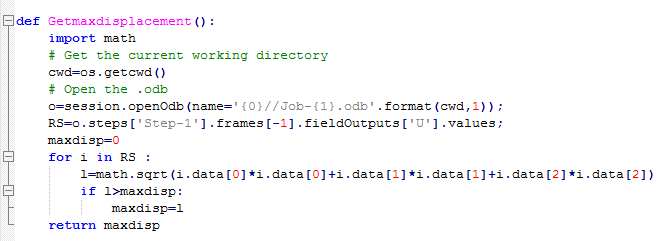
\includegraphics[width = .9\textwidth]{4.png} 
\caption{Plate单元分片实验位移结果} 
\label{f4} 
\end{figure},可见位移$w$准确,误差在浮点数范围内,以7号节点为例:

\begin{equation}
\begin{array}{c}
w_{7}=x_{7}^{2}-\nu y_{7}^{2}=0.25\\
\theta_{x7}=-2\nu y_{7}=0\\
\theta_{y7}=-2x_{7}=-1
\end{array}\label{eq19}
\end{equation}
从$\theta_{x}$上的误差上来看,误差基本上在$10^{-16}$量级上,为计算机浮点数的误差

\subsection{收敛率计算}

考虑一个正方形板,$W=L=2,t=1$,其中$E=3\times10^{7},\nu=0.3,t=1$如图\ref{f5}所示:

\begin{figure}[H]
\centering  
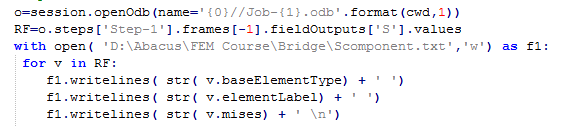
\includegraphics[width = .5\textwidth]{5.png} 
\caption{Plate收敛率计算示意图} 
\label{f5} 
\end{figure}在中心点施加一个集中力($-z$方向)$P=10^{5}$,因此只需要在对应的节点施加这样一个力即可,然后分别考虑划分4,16,64和256个等大小的矩形板单元进行计算(对应单元尺寸$h=1,0,5,0.25,0.0.125$),相应的输入文件用data.m生成,分别为:Plate4ele.dat,Plate16ele.dat和Plate64ele.dat,Plate256ele.dat,计算相应的节点位移$w^{e}$与理论结果进行比较:

\begin{equation}
w=\frac{16P}{D\pi^{4}}\sum_{m=0}^{\infty}\sum_{n=0}^{\infty}\frac{(-1)^{(}m+n)}{\left((2m+1)^{2}+(2n+1)^{2}\right)^{2}}\sin\frac{m\pi x}{2}\sin\frac{n\pi y}{2}\label{eq20}
\end{equation}
计算误差范数:

\begin{equation}
error=(\int_{0}^{L}\int_{0}^{W}(w^{e}-w)^{2}dxdy)^{\frac{1}{2}}\label{eq21}
\end{equation}
由于$w$至少是4次场,所以该积分至少需要采用16{*}16的Gauss积分才能准确积分,得到计算结果如图\ref{f6}所示,并作出误差范数和单元尺寸的对数图

\begin{figure}[H]
\centering  
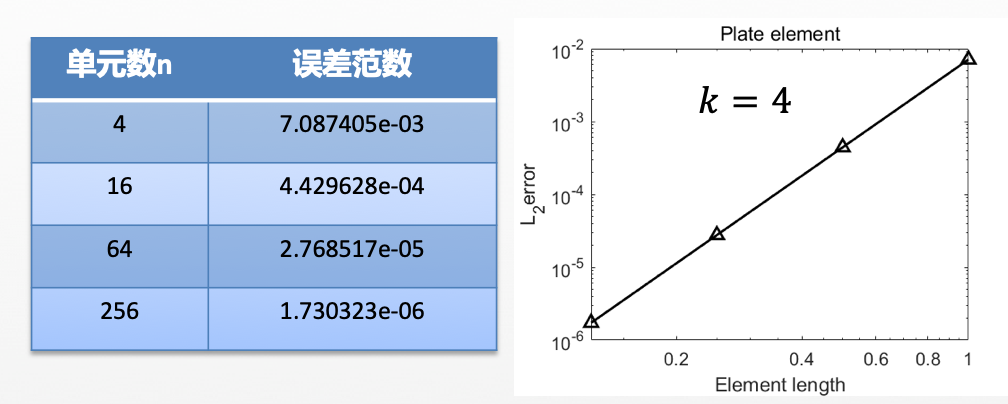
\includegraphics[width = .5\textwidth]{6.png} 
\caption{Plate收敛率计算结果} 
\label{f6} 
\end{figure}可见板单元的挠度$w$是4阶收敛的,因为其构造挠度的多项式是3次完备的。

\section{9节点平面亚参元(Subparameter Element)}

\subsection{9节点平面亚参元基本公式}

我们这里采用的9节点平面亚参元,其母单元示意图如图\ref{f7}所示:

\begin{figure}[H]
\centering  
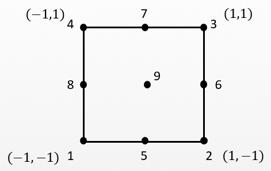
\includegraphics[width = .5\textwidth]{7.png} 
\caption{9节点平面亚参元母单元示意图} 
\label{f7} 
\end{figure}其坐标差值点为1,2,3,4四个节点,而位移差值采用1-9九个节点:

\begin{equation}
\begin{aligned}x & =\sum_{I=1}^{4}N_{I}^{\prime}x_{I}\\
y & =\sum_{I=1}^{4}N_{I}^{\prime}y_{I}\\
\theta & =\sum_{K=1}^{9}N_{K}\theta_{K}
\end{aligned}
\label{eq22}
\end{equation}
其中$N_{I}^{\prime}=\frac{1}{4}\left(1+\xi_{I}\xi\right)\left(1+\eta_{I}\eta\right)$,而:

\begin{equation}
\begin{array}{c}
N_{1}=\frac{1}{4}\xi\eta(\xi-1)(\eta-1)\\
N_{2}=\frac{1}{4}\xi\eta(\xi+1)(\eta-1)\\
N_{3}=\frac{1}{4}\xi\eta(\xi+1)(\eta+1)\\
N_{4}=\frac{1}{4}\xi\eta(\xi-1)(\eta+1)\\
N_{5}=\frac{1}{2}\eta(\eta-1)(1-\xi^{2})\\
N_{6}=\frac{1}{2}\xi(\xi+1)(1-\eta^{2})\\
N_{7}=\frac{1}{2}\eta(\eta+1)(1-\xi^{2})\\
N_{8}=\frac{1}{2}\xi(\xi-1)(1-\eta^{2})\\
N_{9}=(1-\xi^{2})(1-\eta^{2})
\end{array}\label{eq23}
\end{equation}


\subsection{9节点平面亚参元的应力应变以及刚度阵构造}

其余过程和4Q单元一致,首先应变由位移差值(\ref{eq22})可以得到:

\begin{equation}
\begin{array}{c}
\bm{\varepsilon^{e}}=\sum_{i=1}^{9}\bm{B_{i}d_{i}}\\
\bm{d_{i}}=\begin{bmatrix}u_{i}\\
v_{i}
\end{bmatrix}\\
\bm{B_{i}}=\begin{bmatrix}\frac{\partial N_{i}}{\partial x} & 0\\
0 & \frac{\partial N_{i}}{\partial y}\\
\frac{\partial N_{i}}{\partial y} & \frac{\partial N_{i}}{\partial x}
\end{bmatrix}
\end{array}\label{eq24}
\end{equation}
利用雅可比矩阵得到物理空间坐标和母单元坐标的转换关系(但这里的坐标利用的是4节点差值),进而得到单元刚度阵($18\times18$):

\begin{equation}
\bm{K^{e}}=\int_{-1}^{1}\int_{-1}^{1}\bm{B^{T}DB}det|\bm{J}|{\rm d}\xi{\rm d}\eta\label{eq25}
\end{equation}
采用Skyline的方式深书写到程序中,并且采用 $3\times3$的Gauss积分计算每一个元素。

而相应的节点等效力由公式:

\begin{equation}
\boldsymbol{f}^{e}=\int_{\Gamma_{t}^{e}}\boldsymbol{N}^{e\mathrm{T}}\overline{\boldsymbol{t}}\mathrm{d}\Gamma+\int_{\Omega^{e}}\boldsymbol{N}^{e\mathrm{T}}\boldsymbol{b}\mathrm{d}\Omega\label{eq26}
\end{equation}
计算

\subsection{输入文件格式和自由度约束}

平面9节点亚参元的输入文件和4Q单元类似,其后三个转动自由度可以在Stap++中默认设置为1,然后可以不需要在输入文件中体现,而对于一般的平面问题,我们可以不锁死z方向的自由度,但是为了求解简单,一般我们可以把坐标系的xy设置为单元所在的面,这样我们可以把z方向的自由度(bcode{[}2{]})设置为1,这样对应的平面9节点亚参元的总自由度为18。

关于节点信息的输入,严格来说,我们可以用1,2,3,4号节点自动生成节点5-9的坐标,但是在Nodelist中需要出现5-9对应的节点号,由于在Stap++中实现自动添加节点的功能还没有扩展(这也是可以继续扩展的方向),因此我们还是需要在输入文件中输入5-9号节点,只是相应的坐标全部可以写为0,然后在Stap++中会计算其相应的坐标赋值给XYZ

材料和受力和一般的单元输入格式一致,而单元对应的节点号部分应该按照图\ref{f7}对应的节点编号顺序填,图\ref{f8}展示了一个9节点亚参元的输入文件格式:

\begin{figure}[H]
\centering  
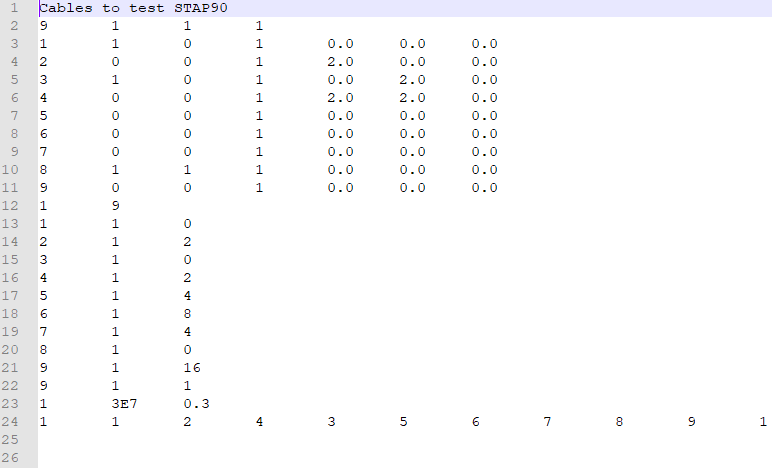
\includegraphics[width = .8\textwidth]{8.png} 
\caption{1个9节点亚参元的输入文件格式} 
\label{f8} 
\end{figure}

\subsection{分片测试}

先考虑考虑一个平板的一端(沿着xy平面),长宽:$W=L=2$,其材料参数:$E=3\times10^{7},\nu=0.3$,其受到$x$方向的一个均匀拉力$\sigma=9$的情况,如图\ref{f9}所示:

\begin{figure}[H]
\centering  
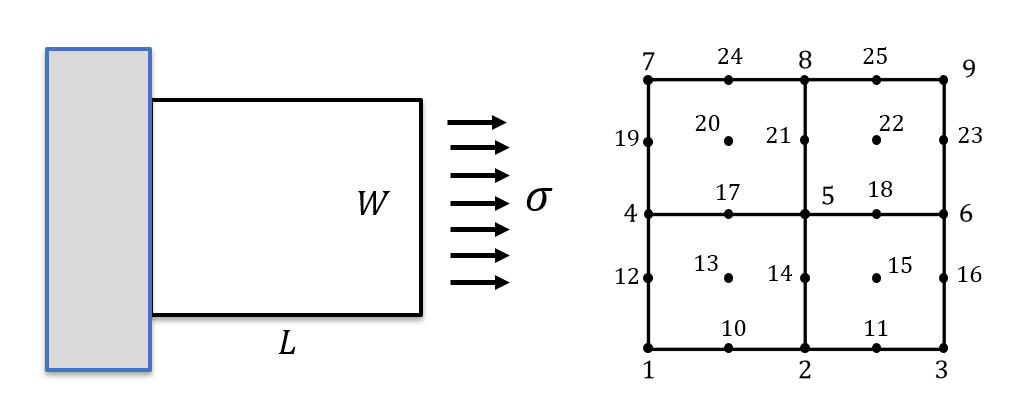
\includegraphics[width = .5\textwidth]{9.png} 
\caption{9节点平面亚参元的分片测试1示意图} 
\label{f9} 
\end{figure}并且我们划分4个等大的单元,节点划分如图\ref{f9}所示,其中平板的一段被约束住(即节点1,7,12,19被约束住$x$方向自由度,而4号节点约束住$x,y$方向自由度);利用节点力等效公式(\ref{eq26})我们可以得到在该情况下(对于矩形单元)的节点等效力为:$f_{ix}|_{\Gamma}=\frac{\sigma h}{2}\int_{-1}^{1}N_{i}(\xi=1){\rm d\eta}$(其中$h$为单元的长度)

\begin{equation}
\begin{array}{c}
f_{2x}=f_{4x}=\frac{1}{6}\sigma h\\
f_{6x}=\frac{2}{3}\sigma h
\end{array}\label{eq27}
\end{equation}
注意这里的1-9对应的是母单元的编号,具体的编号要根据Location matrix对应的世纪编号来;相应的具体输入文件利用matlab程序Subpara\_force.m生成,具体输入文件请见Subparapatchtest.dat,程序计算的求解结果如图\ref{f10}所示:

\begin{figure}[H]
\centering  
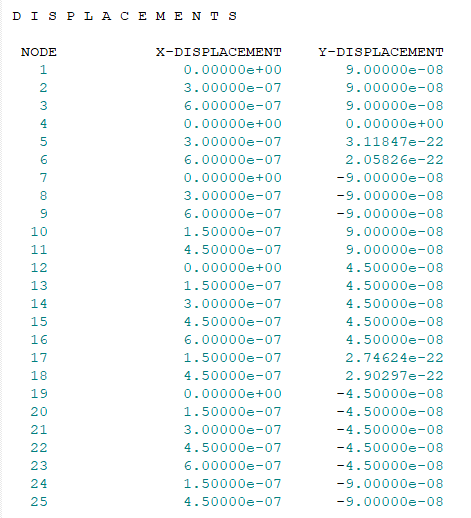
\includegraphics[width = .5\textwidth]{10.png} 
\caption{9节点平面亚参元的分片测试1结果} 
\label{f10} 
\end{figure}其与理论的结果(单轴拉伸):

\begin{equation}
\begin{array}{c}
u=\frac{\sigma}{E}x\\
v=-\frac{\nu\sigma}{E}(y-1)
\end{array}\label{eq28}
\end{equation}
相比较,从5号节点的$y$方向位移,可以看出其误差基本在计算机浮点数范围$(10^{-22})$内,因此通过分片测试1;

进一步的提高分片测试的阶次,给平板一个沿着$x$方向均匀拉伸的体积力$b_{x}=a=9$,其余参数不变,如图\ref{f11}所示:

\begin{figure}[H]
\centering  
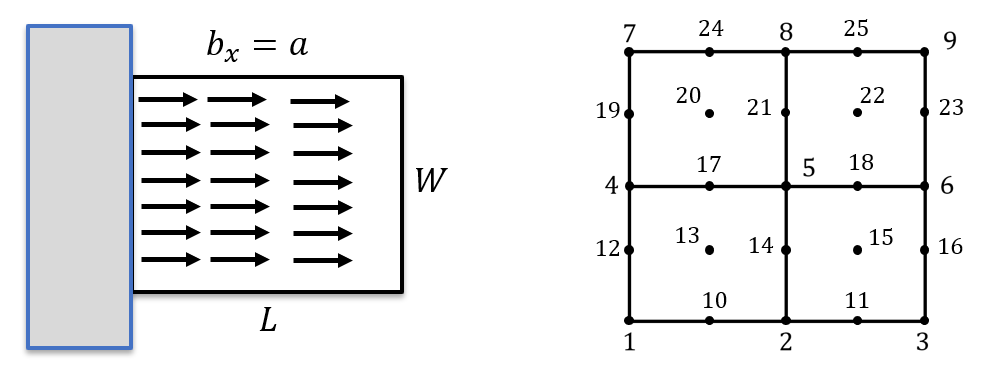
\includegraphics[width = .5\textwidth]{11.png} 
\caption{9节点平面亚参元的分片测试1示意图} 
\label{f11} 
\end{figure}

同样利用节点力等效公式(\ref{eq26}),我们可以得到(对于矩形单元)每个单元等效的节点力为:$f_{ix}=\frac{ah^{2}}{4}\int_{-1}^{1}\int_{-1}^{1}N_{i}{\rm d}\xi{\rm d\eta}$(其中$h$为单元的长度)

\begin{equation}
\begin{array}{c}
f_{1x}=f_{2x}=f_{3x}=f_{4x}=\frac{ah^{2}}{36}\\
f_{5x}=f_{6x}=f_{7x}=f_{8x}=\frac{ah^{2}}{9}\\
f_{9x}=\frac{4ah^{2}}{9}
\end{array}\label{eq29}
\end{equation}
其余的输入文件文件部分和Subparapatchtest.dat相同,见Subparapatchtest2.dat文件;程序的计算求解结果如图\ref{12}所示:

\begin{figure}[H]
\centering  
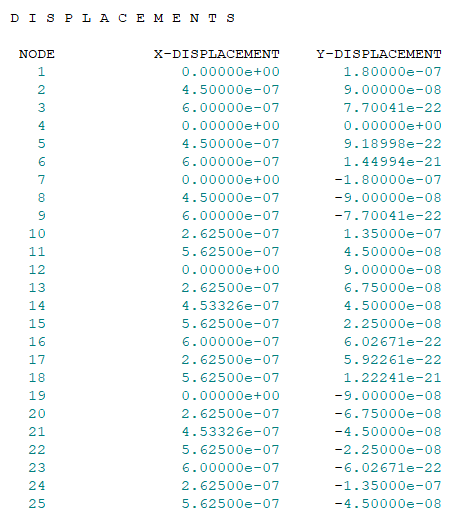
\includegraphics[width = .5\textwidth]{12.png} 
\caption{9节点平面亚参元的分片测试2结果} 
\label{f12} 
\end{figure}其与理论结果:

\begin{equation}
\begin{array}{c}
u=\frac{a}{E}(2x-\frac{x^{2}}{2})\\
v=-\frac{a\nu}{E}(2-x)(y-1)
\end{array}\label{eq30}
\end{equation}
比较的误差在计算浮点数范围$(10^{-22})$,因此其能通过分片测试2,所以其收敛率至少为3。

\subsection{收敛率计算}

将分片测试2中的均匀体积力改为一个沿 $x$方向线性分布体力的情况:$b_{x}=ax(a=9)$,其余几何参数,材料参数以及单元划分不变,如图\ref{f13}所示:

\begin{figure}[H]
\centering  
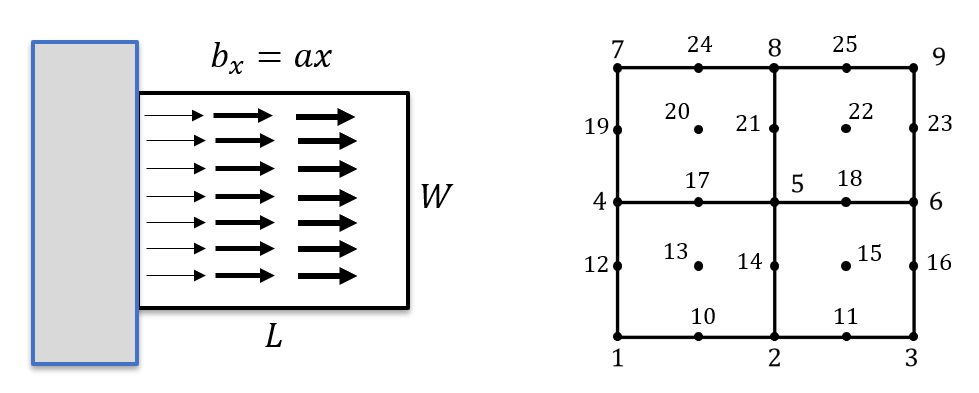
\includegraphics[width = .5\textwidth]{13.png} 
\caption{9节点平面亚参元收敛率计算示意图} 
\label{f13} 
\end{figure}

同样利用节点力等效公式(\ref{eq26}),我们可以得到(对于矩形单元)每个单元等效的节点力为:$f_{ix}=\frac{ah^{2}}{4}\int_{-1}^{1}\int_{-1}^{1}N_{i}{\rm (\frac{x_{1}+x_{2}}{2}+\frac{h}{2}\xi)d}\xi{\rm d\eta}$(其中$x_{1}$和$x_{2}$为母单元中1,2号节点对应物理空间的坐标,$h$为单元长度)

\begin{equation}
\begin{array}{c}
f_{1x}=f_{4x}=\frac{ah^{2}}{36}(\frac{x_{1}+x_{2}}{2}-\frac{h}{2})\\
f_{2x}=f_{3x}=\frac{ah^{2}}{36}(\frac{x_{1}+x_{2}}{2}+\frac{h}{2})\\
f_{5x}=f_{7x}=\frac{ah^{2}}{9}\frac{x_{1}+x_{2}}{2}\\
f_{6x}=\frac{ah^{2}}{9}(\frac{x_{1}+x_{2}}{2}+\frac{h}{2})\\
f_{8x}=\frac{ah^{2}}{9}(\frac{x_{1}+x_{2}}{2}-\frac{h}{2})\\
f_{9x}=\frac{4ah^{2}}{9}\frac{x_{1}+x_{2}}{2}
\end{array}\label{eq31}
\end{equation}
注意这里的1-9对应的是母单元的编号,具体的编号要根据Location matrix对应的世纪编号来;相应的具体输入文件利用matlab程序Subpara\_force.m生成;我们分别计算划分1,4,16和64个单元时的结果(对应单元尺寸$h=2,1,0,5,0.25$),具体输入文件请见Subpara1ele.dat,Subpara4ele.dat,Subpara16ele.dat和Subpara64ele.dat;计算相应的节点位移$w^{e}$与理论结果进行比较:

\begin{equation}
\begin{array}{c}
u=\frac{3}{2E}(12x-x^{3})\\
v=\frac{9\nu}{2E}(x^{2}-4)(y-1)
\end{array}\label{eq32}
\end{equation}
我们这里计算$x$方向位移的误差范数:

\begin{equation}
error=(\int_{0}^{L}\int_{0}^{W}(u^{e}-u)^{2}dxdy)^{\frac{1}{2}}\label{eq33}
\end{equation}
由于$u$是三次场,所以至少要用9{*}9节点Gauss积分,得到的计算结果如图\ref{f14}所示:

\begin{figure}[H]
\centering  
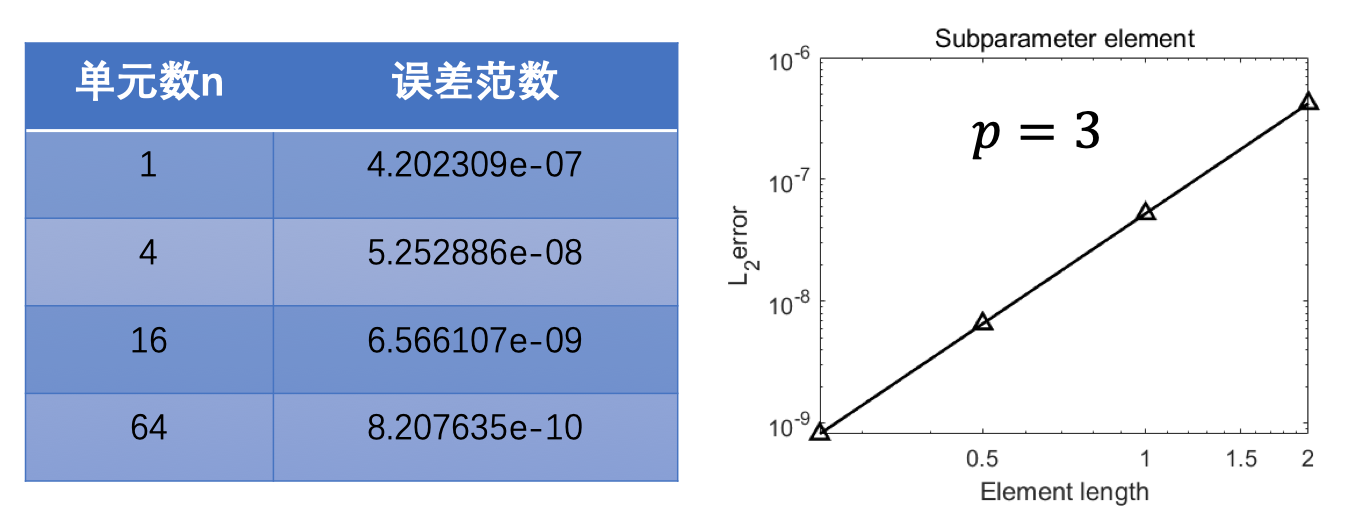
\includegraphics[width = .5\textwidth]{14.png} 
\caption{9节点平面亚参元收敛率计算结果} 
\label{f14} 
\end{figure}可见其位移的收敛率为3,和分片实验的结果一致,因为其位移差值能够精确重构2次多项式。

\section{无限单元(Infinite element)}

\subsection{无限单元的基本公式}

我们这里采用的是4节点平面等参无限单元(之后简称为无限单元);其主要适用于无限大问题的求解,其核心的思想是利用两个参考点$\text{{\rm C}}$和${\rm C_{1}}$把边界点${\rm P}$和${\rm P_{1}}$还有对称的参考点$\text{{\rm Q}和\ensuremath{{\rm Q_{1}}\text{把无穷原点映射到母单元中\ensuremath{\xi=1}}}}$的两个点;最终在母单元中${\rm P},{\rm Q},{\rm R}$和${\rm P}_{1},{\rm Q_{1}},{\rm R_{1}}$对应平行与$\xi$轴的两条边,因此我们只需要构造一种一维差值$(\xi\text{方\text{向}})$能够满足把无穷远R点$(x\to\infty)$映射到$\xi=1$即可,如图\ref{f15}所示:

\begin{figure}[H]
\centering  
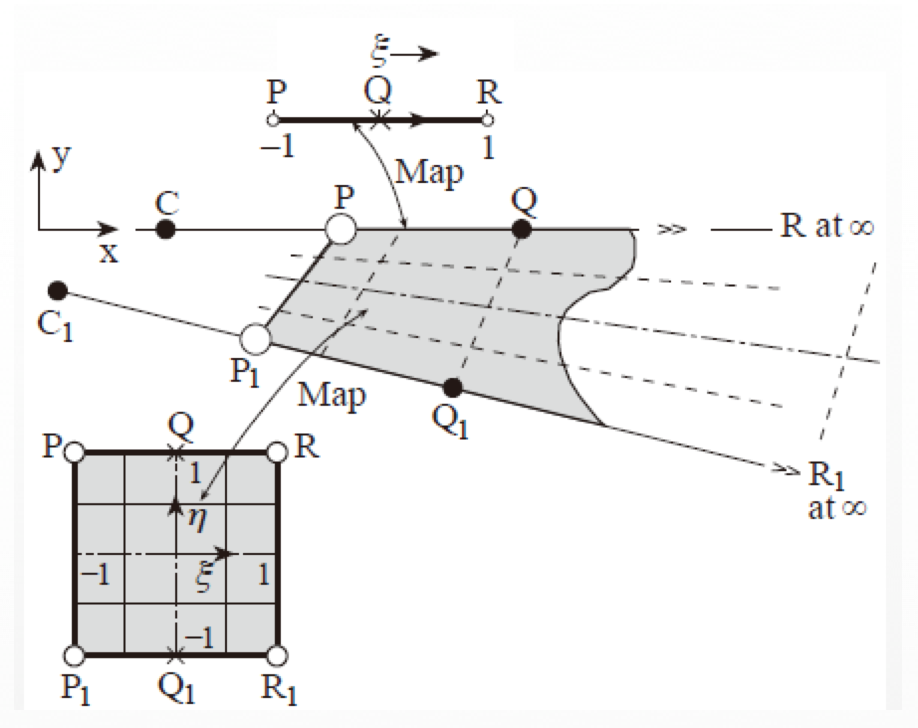
\includegraphics[width = .6\textwidth]{15.png} 
\caption{无限单元映射关系示意图} 
\label{f15} 
\end{figure}首先对于$\xi$方向的差值:

\begin{equation}
\begin{array}{c}
x=\text{\ensuremath{\overline{N}_{C}x_{C}+\overline{N}_{Q}x_{Q}}}\\
\overline{N}_{C}=-\frac{\xi}{1-\xi}\\
\overline{N}_{Q}=1+\frac{\xi}{1-\xi}
\end{array}\label{eq34}
\end{equation}
其可以使得P点从物理空间中的$x=\frac{x_{C}+x_{Q}}{2}$映射到$\xi=-1$,使得Q点从物理空间中的$x=x_{Q}$映射到$\xi=0$,使得R点从物理空间中的$x\to\infty$映射到$\xi=1$,而$\eta$方向的差值可直接采用一般的两节点线性差值:$N_{1}=\frac{1}{2}\eta(1+\eta),N_{0}=\frac{1}{2}\eta(1-\eta)$,于是整个4节点无限单元的形函数和差值关系为:

\begin{equation}
\begin{array}{c}
x=\sum_{i=1}^{4}N_{i}^{*}x_{i}\\
N_{1}^{*}=N_{1}(\eta)\overline{N}_{C}\\
N_{2}^{*}=N_{1}(\eta)\overline{N}_{Q}\\
N_{3}^{*}=N_{0}(\eta)\overline{N}_{C}\\
N_{4}^{*}=N_{0}(\eta)\overline{N}_{Q}
\end{array}\label{eq35}
\end{equation}
其中$i=1$对应C,$i=2$对应Q,$i=3$对应${\rm C_{1}}$,$i=4$对应$Q_{1}$。

\subsection{无限单元的应力应变以及刚度阵构造}

其余有关应力和刚度阵的后续推导和平面4节点等参元一致,但是由于形函数不同(分式多项式),会导致形函数的导数会有变化:

\begin{equation}
\begin{array}{ll}
{\frac{\partial N_{1}^{*}}{\partial\xi}=-\frac{1}{2}\frac{(1+\eta)}{(1-\xi)^{2}}} & {\frac{\partial N_{1}^{*}}{\partial\eta}=-\frac{1}{2}\frac{\xi}{1-\xi}}\\
{\frac{\partial N_{2}^{*}}{\partial\xi}=\frac{1}{2}\frac{(1+\eta)}{(1-\xi)^{2}}} & {\frac{\partial N_{2}^{*}}{\partial\eta}=\frac{1}{2}\left(1+\frac{\xi}{1-\xi}\right)}\\
{\frac{\partial N_{3}^{*}}{\partial\xi}=-\frac{1}{2}\frac{(1-\eta)}{(1-\xi)^{2}}} & {\frac{\partial N_{3}^{*}}{\partial\eta}=\frac{1}{2}\frac{\xi}{1-\xi}}\\
{\frac{\partial N_{4}^{*}}{\partial\xi}=\frac{1}{2}\frac{(1-\eta)}{(1-\xi)^{2}}} & {\frac{\partial N_{4}^{*}}{\partial\eta}=-\frac{1}{2}\left(1+\frac{\xi}{1-\xi}\right)}
\end{array}\label{eq36}
\end{equation}
从而代入到$\bm{B}$矩阵的计算中:

\begin{equation}
\begin{array}{cc}
[\boldsymbol{B}]=\left[\begin{array}{cc}
{\frac{\partial N_{i}^{*}}{\partial x}} & {0}\\
{0} & {\frac{\partial N_{i}^{*}}{\partial y}}\\
{\frac{\partial N_{i}^{*}}{\partial y}} & {\frac{\partial N_{i}^{*}}{\partial x}}
\end{array}\right]=[J]^{-1}\left[GN^{*}\right] & [\mathbf{J}]=\left[\begin{array}{cc}
{\frac{\partial x}{\partial\xi}} & {\frac{\partial y}{\partial\xi}}\\
{\frac{\partial x}{\partial\eta}} & {\frac{\partial y}{\partial\eta}}
\end{array}\right]\end{array}\label{eq37}
\end{equation}
进一步由公式(\ref{eq25})计算刚度阵列,程序中采用$2\times2$的Gauss积分(但是由于这里雅可比矩阵中存在分式多项式,因此Gauss积分不一定能够做到准确积分)计算并且用Skyline的方式存储。

而其余的节点力等效和Gauss点应力计算和4Q单元一致,程序实现上的思路也一致,只是需要把形函数改为(\ref{eq35})

\subsection{无限单元的收敛性分析}

首先无限单元作为物理尺寸无限大的单元无法像常规的单元一样用单元的尺寸来考虑收敛率,但是从等参元的基本性质出发,无限单元是满足等参元的相容性和连续性:(因为其对应的节点C,Q不是有限单元边界上的点P),于此同时其同样满足刚体位移条件:

\begin{equation}
\sum_{i=1}^{4}N_{i}^{*}=1\label{eq38}
\end{equation}
因此该单元是收敛的。但是需要注意,由于无限单元节点的特殊性,这使得输入文件的构造变得很困难,首先需要给定有限单元的边界,然后去寻找关于边界的对称点,这对于程序上实现会有一些难度。
\section{Euler-Bernoulli Beam单元}
\subsection{单元构造}
每个梁单元有两个节点首先确定梁单元的位移向量与载荷向量。规定沿梁的轴线方向为x方向,单元的位移向量与载荷向量可以表示为:
\begin{equation} 
d^{e}=\left(\begin{array}{llllllllllll}{u_{x 1}} & {u_{y 1}} & {u_{z 1}} & {u_{x 1}} & {u_{y 1}} & {u_{z 1}} & {u_{x 2}} & {u_{y 2}} & {u_{z 2}} & {\theta_{x 2}} & {\theta_{y 2}} & {\theta_{y 3}}\end{array}\right)^{T}
 \end{equation}
\begin {equation} 
f^{e}=\left(\begin{array}{cccccccccccc}{F_{x 1}} & {F_{y 1}} & {F_{z 1}} & {M_{x 1}} & {M_{y 1}} & {M_{z 1}} & {F_{x 2}} & {F_{y 2}} & {F_{z 2}} & {M_{x 2}} & {M_{y 3}}\end{array}\right)^{T}
 \end {equation}
其中$u$表示位移,$\theta$表示转角,$f$表示剪力,$M$表示弯矩,下标中1,2分别表示两端节点。\par
对于梁单元有四个独立的模态,第一个为轴向拉伸,与杆单元相同,第二个为沿轴扭转,第三四个分别为垂直于轴线的两个方向的弯曲,单元的刚度矩阵如下,矩阵中各元素的值不需要高斯积分,可直接导出。
\begin{equation}
K^e=\left(\begin{array}{cccccccccccc}
   \frac{EA}{l} & 0 & 0 & 0 & 0 & 0 & -\frac{EA}{l} & 0 & 0 & 0 & 0 & 0\\
 & \frac{12EI_z}{l^3} & 0 & 0 & 0 & \frac{6EI_z}{l^2} & 0 & -\frac{12EI_z}{l^3} & 0 & 0 & 0 & \frac{6EI_z}{l^2} \\
 &  & \frac{12EI_y}{l^3} & 0 & -\frac{6EI_z}{l^2} & 0 & 0 & 0 & -\frac{12EI_y}{l^3} & 0 & -\frac{6EI_z}{l^2} & 0 \\
 &  &  & \frac{GJ_z}{I} & 0 & 0 & 0 & 0 & 0 & - \frac{GJ_z}{I} & 0 & 0\\
 &  &  &  & \frac{4EI_y}{l} & 0 & 0 & 0 & \frac{6EI_y}{l} & 0 & \frac{2EI_y}{l} & 0\\
 &  &  &  &  & \frac{4EI_z}{l} & 0 & -\frac{6EI_z}{l} & 0 & 0 & 0 & \frac{2EI_z}{l}\\
 &  \multicolumn{3}{c}{\raisebox{1.3ex}[0pt]{Symmetry}}  &  &  &\frac{EA}{l} & 0 & 0 & 0 & 0 & 0\\
 &  &  &  &  &  &  & \frac{12EI_z}{l^3} & 0 & 0 & 0 & -\frac{6EI_z}{l^2}\\
 &  &  &  &  &  &  &  & \frac{12EI_y}{l^3} & 0 & \frac{6EI_y}{l^2} & 0\\
 &  &  &  &  &  &  &  &  & \frac{GJ_z}{I} & 0 & 0\\
 &  &  &  &  &  &  &  &  &  & \frac{4EI_y}{l} & 0\\
 &  &  &  &  &  &  &  &  &  &  &\frac{4EI_z}{l}\\
\end{array}\right)
\end{equation}
在写出单元刚度阵以及位移向量之后,我们就得到了单元的控制方程:
\begin{equation} 
K^{e} d^{e}=f^{e}
 \end{equation}
这样就可以准备将单元刚度阵组装到总体刚度阵,当然在此之前需要将单元刚度阵做坐标变换,这源自于在全局的坐标系,真实的单元方程是:
\begin{equation} 
K^{e} R d^{e}= R f^{e}
 \end{equation}
因此有
\begin{equation} 
K^{global} = R^T K^{element} R
 \end{equation}
其中R为12*12的矩阵,其中有四个分块,每个分块都为方向余弦阵
\begin{equation} 
R = 
\begin{bmatrix}
A & & & \\
& A & & \\
& & A & \\
& & & A 
\end{bmatrix}
\end{equation}
其中A=
\begin{equation} 
\hat{A}=\left[\begin{array}{lll}{a_{x} a'_{x}} & {a_{x} a'_{y}} & {a_{x} a'_{z}} \\ {a_{y} a'_{x}} & {a_{y} a'_{y}} & {a_{y} a'_{z}} \\ {a_{z} a'_{x}} & {a_{z} a'_{y}} & {a_{z} a'_{z}}\end{array}\right]
 \end{equation}
将如此经过正交变换的单元刚度阵组装到总刚度阵即可
\subsection{梁单元的输入规定}
梁单元的在单元类型中编号为4,需要输入的材料性质包括基本的杨氏模量 E,泊松比$\mu$,另外本工程项目中使用的是空心矩形截面梁,为保证对称性,即保证不移轴,上下壁面的厚度需要相同,左右壁面的厚度需要相同,因此依次输入的参数是:矩形的长和宽(a,b),上下壁面的厚度,左右壁面的厚度,以及一组单位向量(n1,n2,n3)来表征局部坐标系的y轴在全局坐标系中的方向。考虑到桥梁中的梁单元都存在于xz平面,该向量可以被置为(0,1,0)
\subsection{Patch Test}
首先对于梁进行不规则的划分,如下图所示:

梁的总长度为1m,共划分为4个单元,5个节点,分别在$x=0,0.2,0.3,0.5,1$处。
\begin{figure}[H]
\centering
    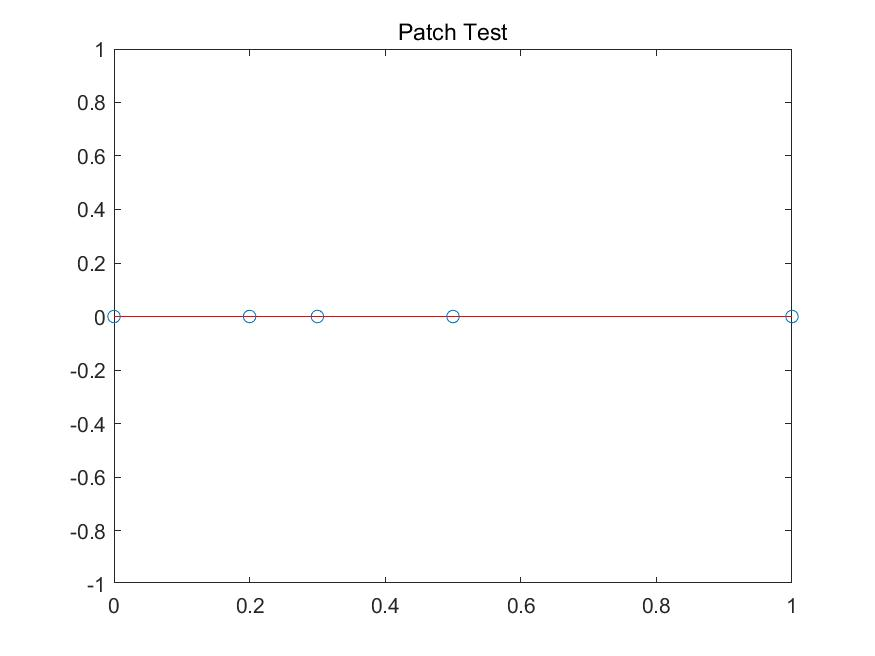
\includegraphics[width=.7\textwidth]{patch_test_beam.jpg}
  \caption{Patch Test}
\end{figure}
由于梁有四个互相独立解耦的模态,对其分别约束测试。\par
首先验证y方向挠度,即z方向弯曲,如下构造精确解。本质边界条件为两端简支,自然边界条件为两边施加等大反向弯矩,梁处于纯弯曲状态且弯矩相等,位移的精确解为:
\begin{equation} 
w= x^{2}- x, \theta=2 x-1
 \end{equation}
分片试验结果如下,
\begin{table}[H]
  \centering
  \caption{DISPLACEMENT-WZ}
    \begin{tabular}{lcccccc}
\hline
NODE & X-D&Y-D &Z-D &$\theta_X$-D &$\theta_Y$-D&$\theta_Z$-D \\
\hline
1 & 0.000e+00 & 0.000e+00 & 0.000e+00 & 0.000e+00 & 0.000e+00 & -1.000e+01 \\
2 & 0.000e+00 & -1.600e+01 & 0.000e+00 & 0.000e+00 & 0.000e+00 & -6.000e+00 \\
3 & 0.000e+00 & -2.100e+01 & 0.000e+00 & 0.000e+00 & 0.000e+00 & -1.000e+01 \\
4 & 0.000e+00 & -2.500e+01 & 0.000e+00 & 0.000e+00 & 0.000e+00 & 1.237e-15 \\
5 & 0.000e+00 & 0.000e+00 & 0.000e+00 & 0.000e+00 & 0.000e+00 & 1.000e+01 \\
\hline
 \end{tabular}%
\end{table}
之后验证z方向挠度,y方向弯曲,边界条件及载荷相同,位移的精确解也相同,节点和分片方式相同,结果如下
\begin{equation} 
w= x^{2}- x, \theta=2 x-1
 \end{equation}
分片试验结果如下,
\begin{table}[H]
  \centering
  \caption{DISPLACEMENT-WZ}
    \begin{tabular}{lcccccc}
\hline
NODE & X-D&Y-D &Z-D &$\theta_X$-D &$\theta_Y$-D&$\theta_Z$-D \\
\hline
1 & 0.000e+00 & 0.000e+00 & 0.000e+00 & 0.000e+00  & -1.000e+01 & 0.000e+00\\
2 & 0.000e+00 &0.000e+00 &  -1.600e+01 & 0.000e+00  & -6.000e+00& 0.000e+00 \\
3 & 0.000e+00 & 0.000e+00 & -2.100e+01 & 0.000e+00 & -1.000e+01 & 0.000e+00 \\
4 & 0.000e+00 & 0.000e+00 & -2.500e+01 & 0.000e+00  & 9.877e-16 & 0.000e+00\\
5 & 0.000e+00 & 0.000e+00 & 0.000e+00 & 0.000e+00  & 1.000e+01 & 0.000e+00\\
\hline
 \end{tabular}%
\end{table}
x方向位移与杆单元的patch test相同,$\theta_x$方向应满足线性收敛率,结果如下
\begin{table}[H]
  \centering
  \caption{DISPLACEMENT-THETAX}
    \begin{tabular}{lcccccc}
\hline
NODE & X-D&Y-D &Z-D &$\theta_X$-D &$\theta_Y$-D&$\theta_Z$-D \\
\hline
1 & 0.000e+00 & 0.000e+00 & 0.000e+00 & 0.000e+00  & 0.000e+00 & 0.000e+00\\
2 & 0.000e+00 &0.000e+00 &0.000e+00 & 2.000e+00  & 0.000e+00& 0.000e+00 \\
3 & 0.000e+00 & 0.000e+00 & 0.000e+00 & 3.000e+00 & 0.000e+00 & 0.000e+00 \\
4 & 0.000e+00 & 0.000e+00 & 0.000e+00 & 5.000e+00  &0.000e+00 & 0.000e+00\\
5 & 0.000e+00 & 0.000e+00 & 0.000e+00 & 1.000e+01  & 0.000e+00 & 0.000e+00\\
\hline
 \end{tabular}%
\end{table}
\subsection{收敛性分析}
选取悬臂梁,调整重力大小,即均布载荷大小,构造出精确解:
梁单元可以有效重构三次位移场,因此,带有均布载荷的悬臂梁可以较好的反应误差。
\begin{equation} 
w=0.01 x^{4}
 \end{equation}
误差范数采用位移范数,可以表示为
\begin{equation} 
\|e\|^2=\int A\left(u-u^{h}\right)^{2} d x
 \end{equation}
计算收敛率时网格划分如下:
\begin{figure}[H]
\centering
  \subfloat[1element]{%
    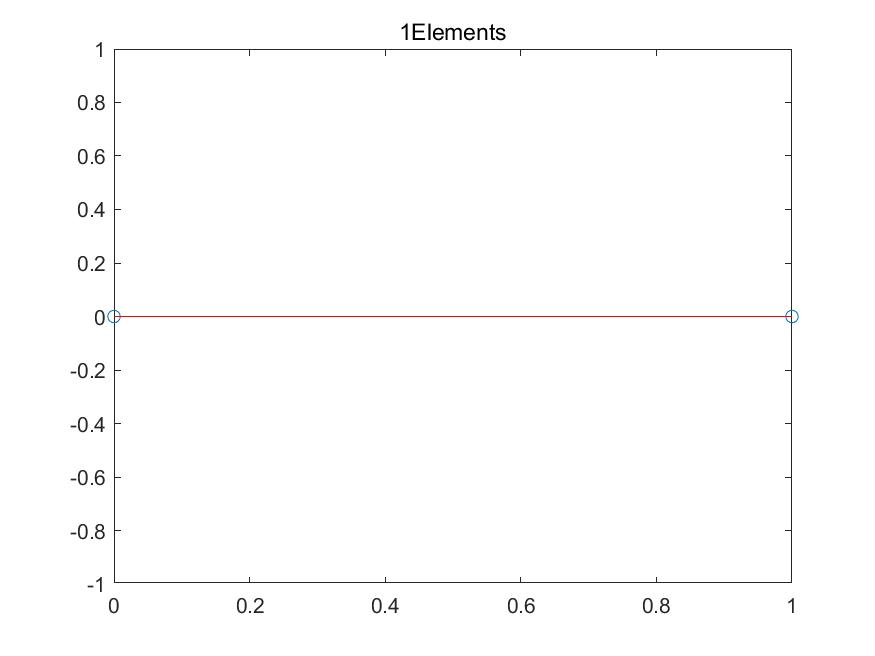
\includegraphics[width=.3\textwidth]{conv_rate0.jpg}}\hfill
  \subfloat[2elements]{%
    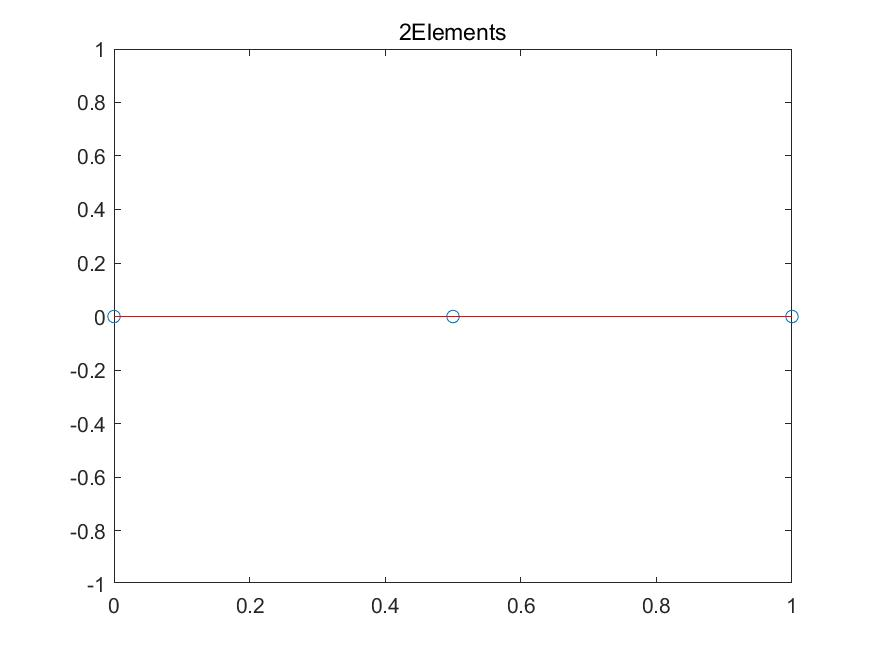
\includegraphics[width=.3\textwidth]{conv_rate1.jpg}}\hfill
\subfloat[3elements]{%
    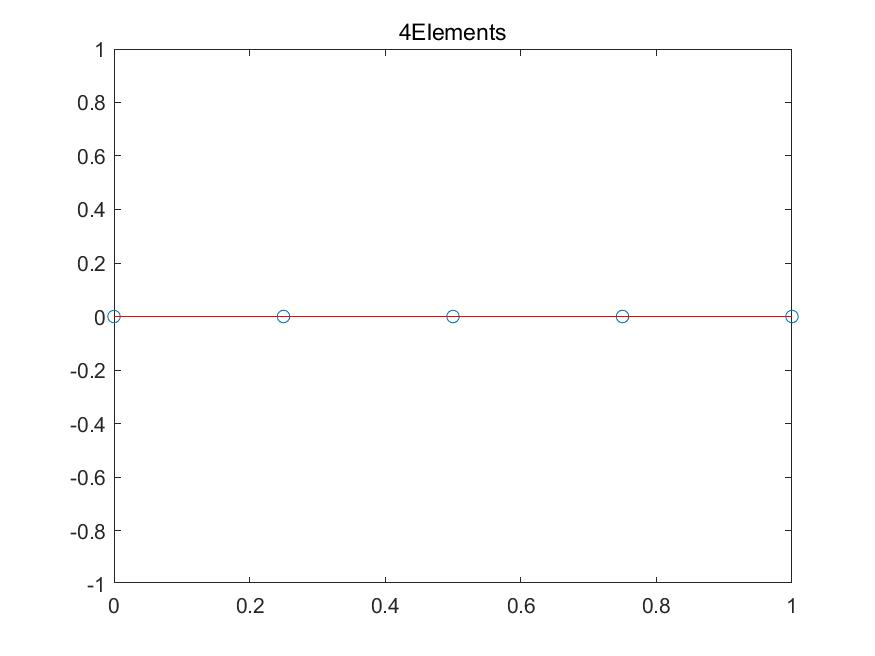
\includegraphics[width=.3\textwidth]{conv_rate2.jpg}}\\

  \subfloat[4elements]{%
    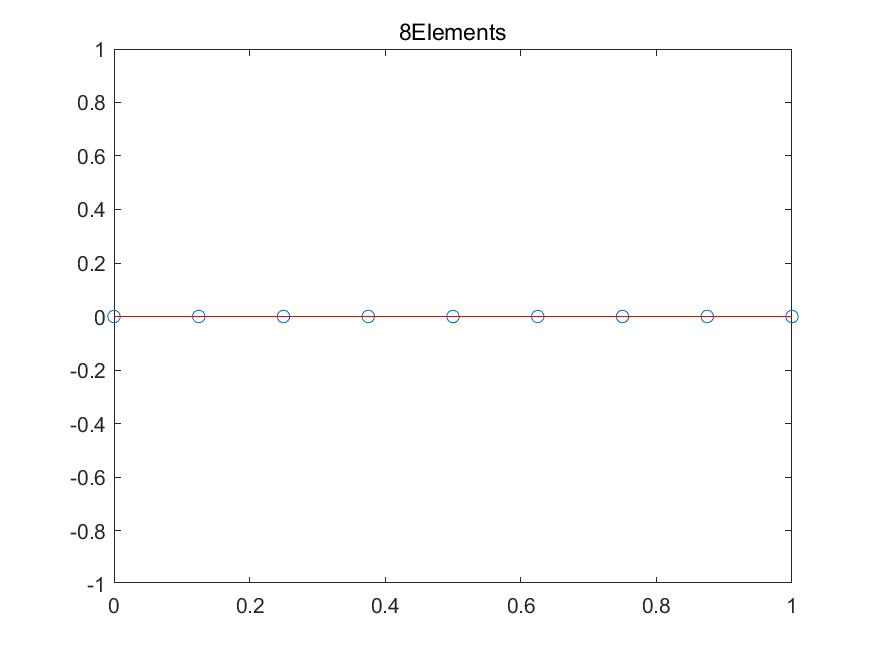
\includegraphics[width=.3\textwidth]{conv_rate3.jpg}}\hfill
 \subfloat[5elements]{%
    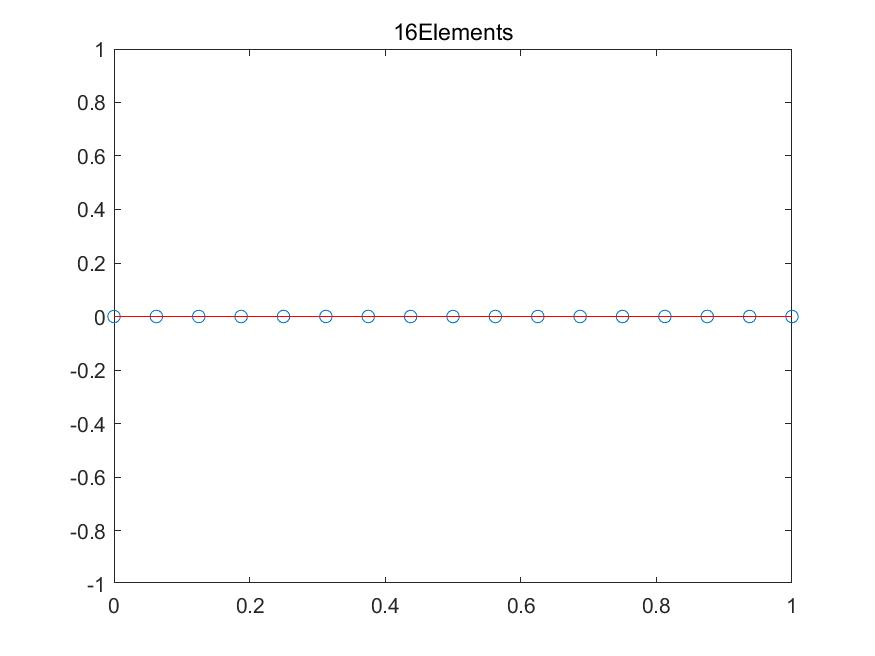
\includegraphics[width=.3\textwidth]{conv_rate4.jpg}}\hfill
\subfloat[6elements]{%
    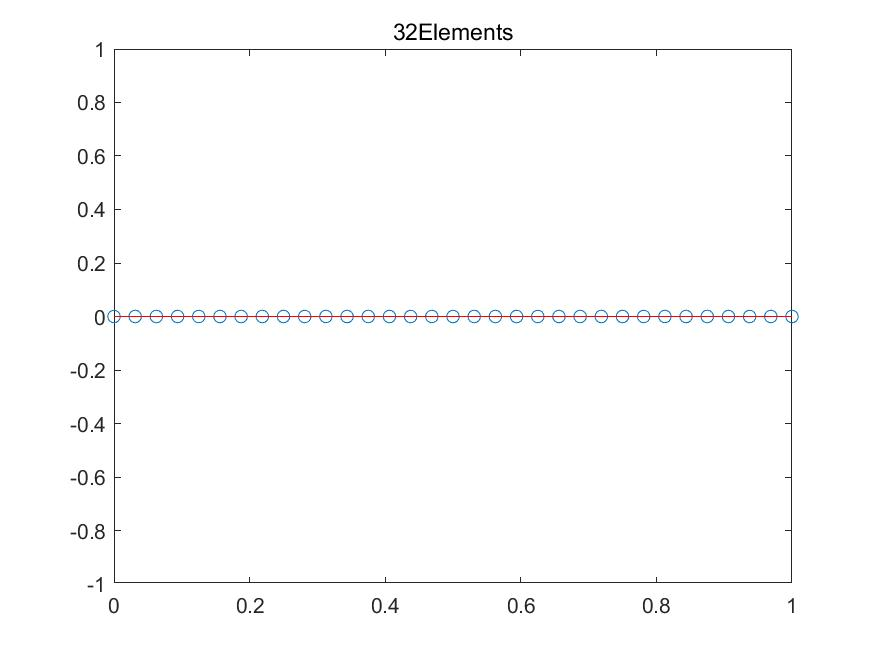
\includegraphics[width=.3\textwidth]{conv_rate5.jpg}}\\
  \caption{Convergence Mesh}\label{fig:2}
\end{figure}
最终收敛率结果如图所示:
\begin{figure}[H]
\centering
    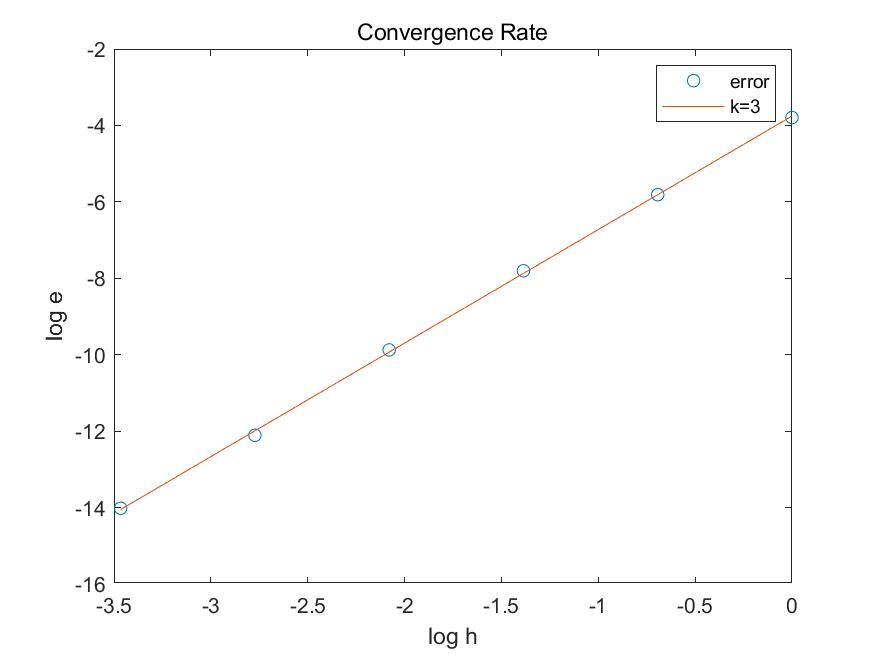
\includegraphics[width=.7\textwidth]{beam_conv_rate.jpg}
  \caption{Convergence Rate}
\end{figure}
\section{Timoshenko Beam}
\subsection{Timoshenko Beam的基本假设}
Euler–Bernoulli梁适用于薄梁,忽略横向剪切变形,横向剪切应力由平衡方程确定,不适用于有效长度较短的梁或组合梁。Timoshenko梁仍然假设与梁轴线垂直的横截面在变形后保持平面(假设为刚性横截面平面),但放松了一些约束,即放弃了直法线假设,采用剪应变沿截面均匀分布的假设,在一定程度上解决了欧拉伯努利梁的问题。
\subsection{Timoshenko Beam 的控制方程}
从变分原理出发有,系统的势能泛函为
\begin{equation} 
\Pi_{P}=\int_{0}^{l} \frac{1}{2} E I\left(\frac{\mathrm{d} \theta}{\mathrm{d} x}\right)^{2} \mathrm{d} x+\int_{0}^{l} \frac{1}{2} \frac{G A}{k} \gamma^{2} \mathrm{d} x-\int_{0}^{l} q w \mathrm{d} x
 \end{equation}
其中,
\begin{equation} 
\varepsilon_{x}=-z \frac{\mathrm{d} \theta}{\mathrm{d} x} \quad \gamma=\frac{\mathrm{d} w}{\mathrm{d} x}-\theta \quad \kappa=-\frac{\mathrm{d} \theta}{\mathrm{d} x}
 \end{equation}
按照有限元格式离散之后可以写成
\begin{equation} 
\begin{aligned} \Pi_{P} &=\int_{0}^{l} \frac{1}{2} E I\left(\frac{\mathrm{d} \theta}{\mathrm{d} x}\right)^{2} \mathrm{d} x+\int_{0}^{l} \frac{1}{2} \frac{G A}{k} \gamma^{2} \mathrm{d} x-\int_{0}^{l} q w \mathrm{d} x \\ &=\sum_{e}\left[\int_{\Omega^{e}} \frac{1}{2} E I\left(\frac{\mathrm{d} \theta}{\mathrm{d} x}\right)^{2} \mathrm{d} x+\int_{\Omega^{e}} \frac{1}{2} \frac{G A}{k} \gamma^{2} \mathrm{d} x-\int_{\Omega^{e}} q w \mathrm{d} x\right] \\ &=\frac{1}{2} \sum_{e}\left(\boldsymbol{d}^{e}\right)^{\mathrm{T}}\left[\left(\boldsymbol{K}_{b}^{e}+\boldsymbol{K}_{s}^{e}\right) \boldsymbol{d}^{e}-f^{e}\right] \end{aligned}
 \end{equation}
其中
\begin{equation} 
\begin{aligned} \boldsymbol{K}_{b}^{e} &=\int_{\Omega^{e}} E I \boldsymbol{B}_{b}^{e \mathrm{T}} \boldsymbol{B}_{b}^{e} \mathrm{d} x \\ \boldsymbol{K}_{s}^{e} &=\int_{\Omega^{e}} \frac{G A}{k} \boldsymbol{B}_{s}^{e \mathrm{T}} \boldsymbol{B}_{s}^{e} \mathrm{d} x \\ \boldsymbol{f}^{e} &=\int_{\Omega^{e}} \boldsymbol{N}^{e \mathrm{T}}\left[\begin{array}{c}{q} \\ {0}\end{array}\right] \mathrm{d} x \end{aligned}
 \end{equation}
根据最小势能原理有
\begin{equation} 
\delta \Pi_{P}=0
 \end{equation}
从而
\begin{equation} 
\begin{array}{l}{E I_{z} \frac{d \kappa_{z}}{d x}+\frac{G A}{k} \gamma_{x y}+\overline{M}_{z k} \delta\left(x-x_{k}\right)=0} \\ {\frac{G A}{k} \frac{d \gamma_{x y}}{d x}+\overline{q}+\overline{N}_{y j} \delta\left(x-x_{j}\right)=0}\end{array}
 \end{equation}
即
\begin{equation} 
\delta \boldsymbol{d}^{\mathrm{T}}\left(\sum_{e} \boldsymbol{L}^{e \mathrm{T}}\left(\boldsymbol{K}_{b}^{e}+\boldsymbol{K}_{s}^{e}\right) \boldsymbol{L}^{e} \boldsymbol{d}-\sum_{e} \boldsymbol{L}^{e \mathrm{T}} \boldsymbol{f}^{e}\right)=0 \quad \forall \boldsymbol{d}_{F}
 \end{equation}
\subsection{有限元离散与插值函数}
我们选取的插值方式为位移转角的一致插值,即考虑两种模式,一种为欧拉伯努利梁,只有弯曲位移,没有剪切位移,另一种为简单修正,只有剪切位移,没有弯曲位移:
\begin{equation} 
\begin{aligned} a &=a_{b}+a_{s} \\ a_{i} &=\left(u_{i}, v_{i}, w_{i}, \varphi_{i}, \theta_{y i}, \theta_{z i}\right)^{T} \\ a_{b} &=\left(a_{b 1}, a_{b 2}\right)^{T} \\ a_{s} &=\left(a_{s 1}, a_{s 2}\right)^{T} \\ a_{b i} &=\left(u_{i}, v_{b i}, w_{b i}, \varphi_{i}, \theta_{y i}, \theta_{z i}\right)^{T} \\ a_{s i} &=\left(0, v_{s i}, w_{s i}, 0,0,0\right)^{T} \end{aligned}
 \end{equation}
对于欧拉伯努利梁的模式,弯曲所产生的变形与转角有如下关系:
\begin{equation} 
\begin{aligned} \frac{d v_{b i}}{d x} &=\theta_{z i} \\ \frac{d w_{b i}}{d x} &=-\theta_{y i} \end{aligned}
 \end{equation}
下面我们选取y,z中的任意方向,进行插值和推导,对于欧拉伯努利梁部分,采用Hermite插值
\begin{equation} 
v_{b}=N_{1} v_{b 1}+N_{2} \theta_{1}+N_{3} v_{b 2}+N_{4} \theta_{4}
 \end{equation}
对于剪切部分,采用两点线性插值
\begin{equation} 
v_{s}=N_{5} v_{s 1}+N_{6} v_{s 2}
 \end{equation}
其中$\xi$为母单元坐标值
\begin{equation} 
\begin{array}{ll}{N_{1}=1-3 \xi^{2}+2 \xi^{3}} & {N_{2}=\left(\xi-2 \xi^{2}+\xi^{3}\right)}l \\ {N_{3}=3 \xi^{2}-2 \xi^{3}} & {N_{4}=\left(\xi^{3}-\xi^{2}\right) l} \\ {N_{5}=1-\xi} & {N_{6}=\xi}\end{array}
 \end{equation}
将插值函数代入有
\begin{equation} 
\boldsymbol{B}_{b}^{e}=\left[\begin{array}{ccc} \frac{\mathrm{d} N_{1}}{\mathrm{d} x} & \ldots & \frac{\mathrm{d} N_{n}}{\mathrm{d} x}\end{array}\right]
 \end{equation}
由于单元内部平衡方程$Q=\frac{d M}{d x}$,欧拉伯努利梁部分与剪力部分有如下关系
\begin{equation} 
\left(\begin{array}{c}{v_{b 2}-v_{b 1}} \\ {v_{s 2}-v_{s 1}}\end{array}\right)=\left(\begin{array}{cc}{\frac{1}{1+b_{z}}} & {\frac{l b_{z}}{2\left(1+b_{z}\right)}} \\ {\frac{b_{z}}{1+b_{z}}} & {-\frac{l b_{z}}{2\left(1+b_{z}\right)}}\end{array}\right)\left(\begin{array}{c}{v_{2}-v_{1}} \\ {\theta_{z 1}+\theta_{z 2}}\end{array}\right)
 \end{equation}
其中,$b_{z} :=\frac{12 E I_{z} k}{G A l^{2}}$,对于矩形截面梁的近似有$k=\frac{6}{5}$。整理之后可以得到,
$\boldsymbol{K} \boldsymbol{d}=\boldsymbol{F}$
其中
\begin{equation} 
\boldsymbol{K}=\frac{E I_{z}}{\left(1+b_{z}\right) l^{3}}\left(\begin{array}{cccc}{12} & {-12} & {6 l} & {6 l} \\ { } & {12} & {-6 l} & {-6 l} \\ { } & { } & {\left(4+b_{z}\right) l^{2}} & {\left(2-b_{z}\right) l^{2}} \\ {[\text {symmetry}]} & & & {\left(4+b_{z}\right) l^{2}} \end{array}\right)
 \end{equation}
考虑所有分量的问题,同时加入扭转以及拉压方向的问题
\begin{equation} 
\boldsymbol{a}=\boldsymbol{a}_{b}+\boldsymbol{a}_{s}
 \end{equation}
有如下刚度阵
\begin{equation}
\setlength{\arraycolsep}{1pt}
\left(\begin{array}{cccccccccccc}
  \frac{EA}{l} & 0 & 0 & 0 & 0 & 0 & -\frac{EA}{l} & 0 & 0 & 0 & 0 & 0\\
 & \frac{12EI_z}{(1+b_z)l^3} & 0 & 0 & 0 & \frac{(1+b_z)6EI_z}{l^2} & 0 & -\frac{12EI_z}{l^3} & 0 & 0 & 0 & \frac{6EI_z}{(2-b_z)l^2} \\
 &  & \frac{12EI_y}{(1+b_y)l^3} & 0 & -\frac{6EI_z}{(1+b_y)l^2} & 0 & 0 & 0 & -\frac{12EI_y}{(1+b_y)l^3} & 0 & -\frac{6EI_z}{(1+b_y)l^2} & 0 \\
 &  &  & \frac{GJ_z}{I} & 0 & 0 & 0 & 0 & 0 & - \frac{GJ_z}{I} & 0 & 0\\
 &  &  &  & \frac{(4+b_y)EI_y}{(1+b_y)l} & 0 & 0 & 0 & \frac{6EI_y}{(1+b_y)l} & 0 & \frac{(2-b_y)EI_y}{(1+b_y)l} & 0\\
 &  &  &  &  & \frac{(4+b_z)EI_z}{(1+b_z)l} & 0 & -\frac{6EI_z}{(1+b_z)l} & 0 & 0 & 0 & \frac{(2-b_z)EI_z}{(1+b_z)l}\\
 &  \multicolumn{3}{c}{\raisebox{1.3ex}[0pt]{Symmetry}}  &  &  &\frac{EA}{l} & 0 & 0 & 0 & 0 & 0\\
 &  &  &  &  &  &  & \frac{12EI_z}{(1+b_z)l^3} & 0 & 0 & 0 & -\frac{6EI_z}{(1+b_z)l^2}\\
 &  &  &  &  &  &  &  & \frac{12EI_y}{(1+b_y)l^3} & 0 & \frac{6EI_y}{(1+b_y)l^2} & 0\\
 &  &  &  &  &  &  &  &  & \frac{GJ_z}{I} & 0 & 0\\
 &  &  &  &  &  &  &  &  &  & \frac{(4-b_y)EI_y}{(1+b_y)l} & 0\\
 &  &  &  &  &  &  &  &  &  &  &\frac{(4-b_y)EI_z}{(1+b_z)l}\\
\end{array}\right)
\end{equation}
同时单元应力的具体计算公式如下:
\begin{equation} 
\begin{aligned} \sigma_{x x} &=E \varepsilon_{x x}=\frac{E\left(u_{2}-u_{1}\right)}{l} \\ \sigma_{x y} &=\frac{G}{k} \gamma_{x y} \\ &=\frac{G}{k l} \frac{b_{z}}{1+b_{z}}\left(\left(v_{2}-v_{1}\right)-\frac{1}{2}\left(\theta_{z 1}+\theta_{z 2}\right) l\right) \\ \sigma_{x z} &=\frac{G}{k} \gamma_{x z} \\ &=\frac{G}{k l} \frac{b_{y}}{1+b_{y}}\left(\left(w_{2}-w_{1}\right)+\frac{1}{2}\left(\theta_{y 1}+\theta_{y 2}\right) l\right) \end{aligned}
 \end{equation}
\subsection{程序实现}
在Stappp程序中新增了Timoshenko单元,在基类Material的基础上派生了CTimoshenkoMaterial类,Timoshenko梁的裁量性质与Beam相同,同时在程序实现时需要注意坐标的转换,我们得出的刚度阵是在单元坐标系中得出的,我们需要将其转换到全局坐标系组装。与Beam单元类似,有
\begin{equation} 
K^{e} R d^{e}= R f^{e}
 \end{equation}
因此有
\begin{equation} 
K^{global} = R^T K^{element} R
 \end{equation}
其中R为12*12的矩阵,其中有四个分块,每个分块都为方向余弦阵
\begin{equation} 
R = 
\begin{bmatrix}
A & & & \\
& A & & \\
& & A & \\
& & & A 
\end{bmatrix}
\end{equation}
其中A=
\begin{equation} 
\hat{A}=\left[\begin{array}{lll}{a_{x} a'_{x}} & {a_{x} a'_{y}} & {a_{x} a'_{z}} \\ {a_{y} a'_{x}} & {a_{y} a'_{y}} & {a_{y} a'_{z}} \\ {a_{z} a'_{x}} & {a_{z} a'_{y}} & {a_{z} a'_{z}}\end{array}\right]
 \end{equation}
将如此经过正交变换的单元刚度阵组装到总刚度阵即可
\subsection{Patch Test}
对于Timoshenko单元,我们考虑其常应变模态为常曲率与常剪应变状态,对于位移与转角有:
\begin{equation} 
\begin{aligned} v &=\frac{1}{2} a x^{2}+c x+d \\ \theta_{z} &=a x+b \end{aligned}
 \end{equation}
注意到此处转角并非单纯位移的积分,因为剪力项对于位移有线性贡献儿对于转角无贡献。这一状态实际上对应于一端集中剪力载荷与弯矩载荷共同作用的悬臂梁。此处选取两种精确解进行patch test的测试。首先为常弯曲状态,即悬臂梁一端施加弯矩。具有如下精确解
\begin{equation} 
w=0.5x^{2}, \theta= x
 \end{equation}
分片试验结果如下:
\begin{figure}[H]
\centering
  \subfloat[1element]{%
    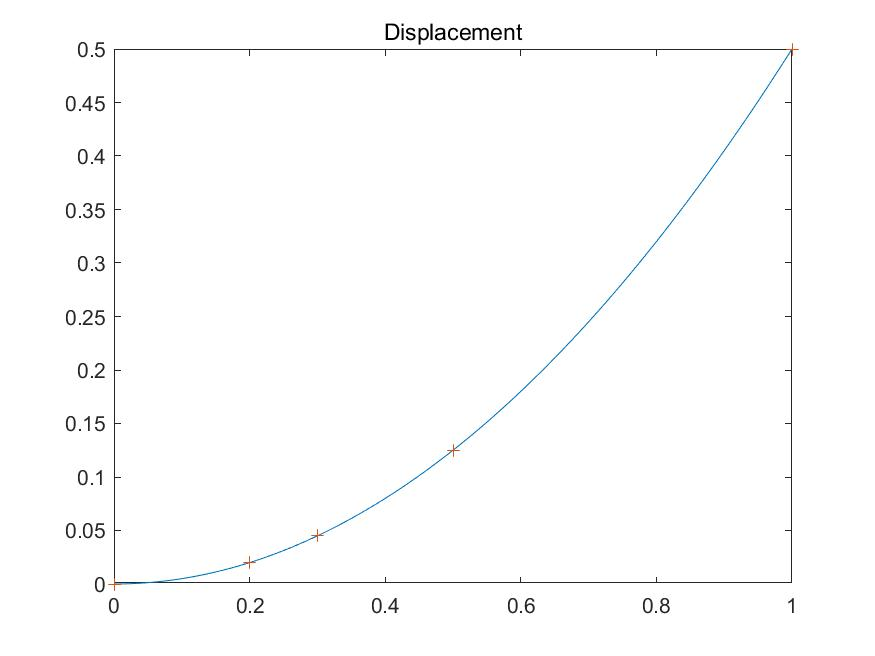
\includegraphics[width=.5\textwidth]{Timo_patch_dis.jpg}}\hfill
  \subfloat[2elements]{%
    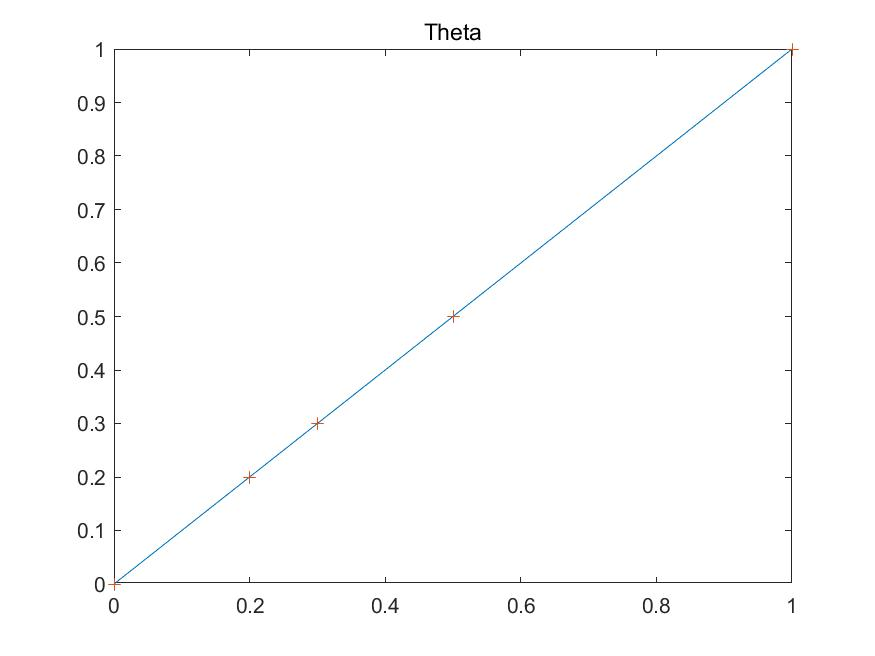
\includegraphics[width=.5\textwidth]{Timo_patch_theta.jpg}}\hfill

  \caption{Timoshenko Beam Patch Test 1}\label{fig:2}
\end{figure}
其次对于纯剪应力状态,精确解为
\begin{equation} 
w=-x^3+3x^{2}+x, \theta= -3x^2+6x
 \end{equation}
分片试验结果如下:
\begin{figure}[H]
\centering
  \subfloat[1element]{%
    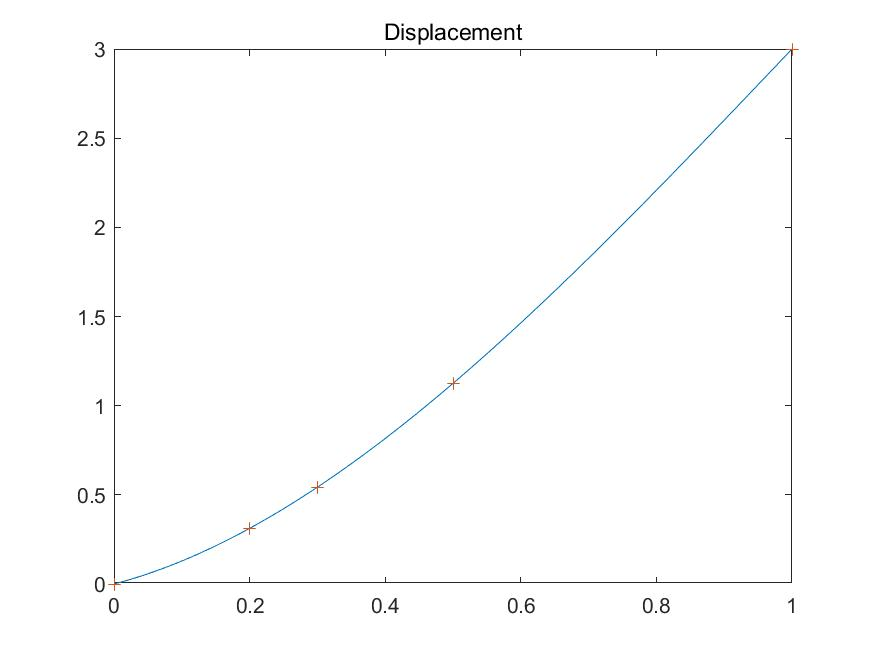
\includegraphics[width=.5\textwidth]{Timo_patch2_dis.jpg}}\hfill
  \subfloat[2elements]{%
    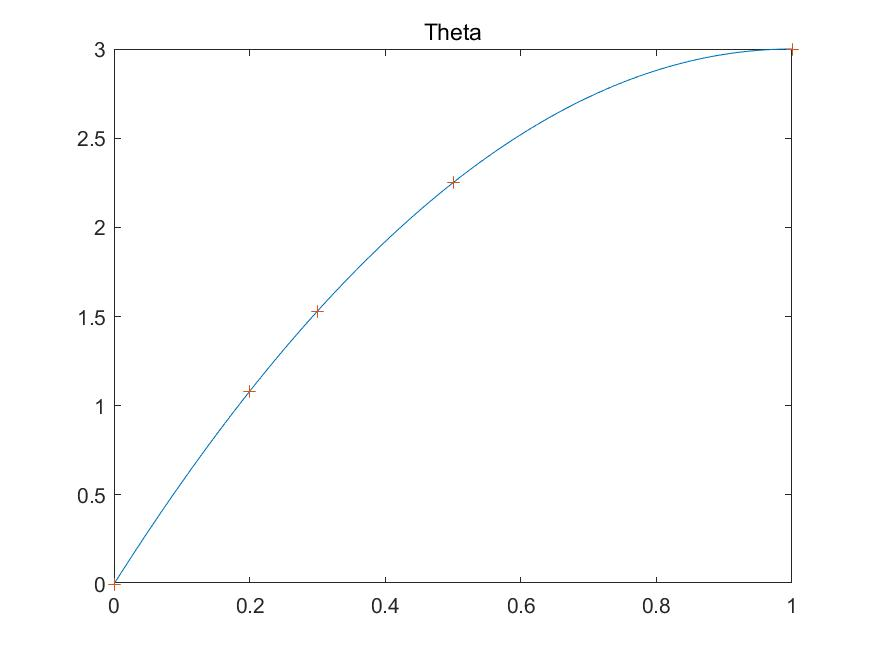
\includegraphics[width=.5\textwidth]{Timo_patch2_theta.jpg}}\hfill

  \caption{Timoshenko Beam Patch Test 2}\label{fig:2}
\end{figure}

\subsection{收敛率验证}
选取均布载荷,对于转角验证收敛率,精确解为三次函数,选取位移范数,收敛率如图
\begin{figure}[H]
\centering
    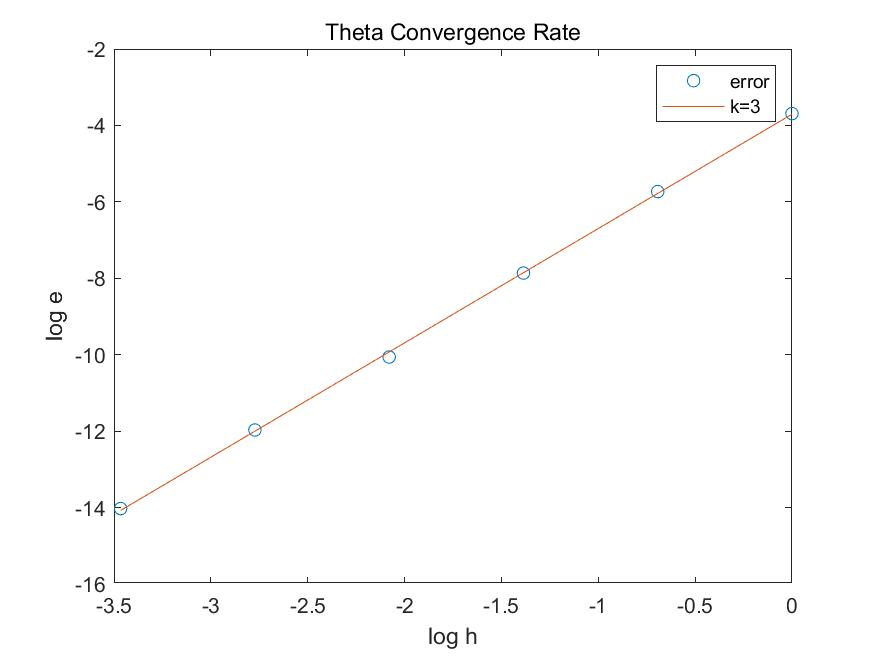
\includegraphics[width=.7\textwidth]{Timobeam_conv_rate.jpg}
  \caption{Convergence Rate}
\end{figure}



%我加在这里了
\section{Shell单元}
\subsection{Shell单元的有限元格式}
本组使用了两种方式建立Shell单元。较为简单的是平板壳单元,它是4Q单元与Plate单元的叠加。其适用范围仅限于矩形平面壳。另一种建立方法则是一般壳体单元,给定节点之后即可对壳的几何形状进行差值,因而适用于一般的曲面壳单元。

所建立的壳单元是4节点的,每个节点的自由度为6,因此壳单元的刚度阵为24阶的。建立平板壳单元即将4Q以及Plate对应位置的刚度阵的元素填充上去。由于是平板壳单元,壳单元的法相均为Z方向,因此$\theta_z=0$,刚度阵中各节点有关z方向转角的项均为零。如此建立的平板壳单元x、y方向的平移自由度与z方向的平移自由度、x、y方向的转动自由度完全解耦。从而,由于使用的4Q单元以及Plate单元均通过了Patch Test,无需再对平板壳单元作检验。

\begin{figure}[h]
	\centering
	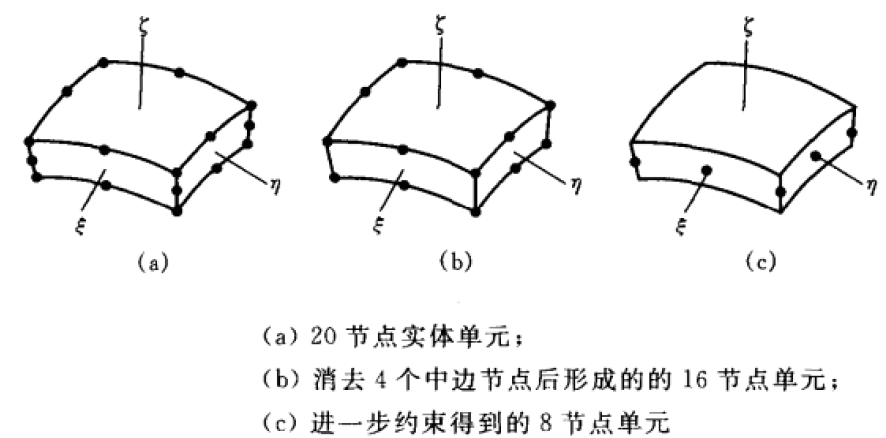
\includegraphics[width=0.65\linewidth]{Shell.png}  
	\caption{曲面壳单元} 
	\label{fig:mcmthesis-logo}
\end{figure}

而一般壳体单元的建立则要从插值开始,映射到母单元,建立应力应变关系从而完成刚度阵的构建。具体如下,第一步建立插值函数。首先根据四个节点坐标可以插值得到壳单元的曲面,使用母单元的坐标表示。对四个节点进行微分以及叉乘计算,可以确定法向量的方向。并由法向量计算出壳单元中每个点与母单元的映射关系。
\begin{center}
$x=\sum_i^4 N_ix_i\quad y=\sum_i^4 N_iy_i\quad z=\sum_i^4 N_iz_i$\\
$\overrightarrow n=(\begin{matrix}\frac{\partial x}{\partial \xi}&\frac{\partial y}{\partial \xi}&\frac{\partial z}{\partial \xi}\end{matrix})\times (\begin{matrix}\frac{\partial x}{\partial \eta}&\frac{\partial y}{\partial \eta}&\frac{\partial z}{\partial \eta}\end{matrix})|_{\xi=\xi_i,\eta=\eta_i}$\\
$\left[\begin{matrix}x\\y\\z\end{matrix}\right]=\sum N_i\{\left[\begin{matrix}x_i\\y_i\\z_i\end{matrix}\right]+\zeta\frac{t}{2}\left[\begin{matrix}l_{3i}\\m_{3i}\\n_{3i}\end{matrix}\right]\}$
\end{center}
其中,$t$是厚度,$l_{3i}$、$m_{3i}$以及$n_{3i}$为各节点法向量分量。局部坐标系的建立可以令局部坐标系中x轴为z轴与全局坐标系的叉乘,之后再用z轴与x轴叉乘得到y轴。第二步计算雅可比矩阵,即直接将$x$、$y$以及$z$针对$\xi$、$\eta$以及$\zeta$求导。在此列出$x$的求导结果,根据对称性,$y$、$z$的结果是类似的。
\begin{center}
$x_{,\xi}=\sum N_{i,\xi}(x_i+\frac{1}{2}\zeta tl_{3i})$\\
$x_{,\eta}=\sum N_{i,\eta}(x_i+\frac{1}{2}\zeta tl_{3i})$\\
$x_{,\zeta}=\sum N_i(\frac{1}{2}tl_{3i})$
\end{center}
第三步建立局部坐标系中应变-位移关系。首先,可以通过插值得到单元任意一点处的位移与节点位移的关系,在此节点的转动自由度是局部坐标系上的$\theta_x$以及$\theta_y$。从而可以得到
\begin{center}
$\left[\begin{matrix}
u_{,\xi}\\u_{,\eta}\\u_{,\zeta}\\v_{,\xi}\\...\\w_{,\zeta}
\end{matrix}\right]=\sum\left[\begin{matrix}
N_{i,\xi}&0&0&-\frac{1}{2}\zeta tN_{i,\xi}l_{2i}&\frac{1}{2}\zeta tN_{i,\xi}l_{1i}\\N_{i,\eta}&0&0&-\frac{1}{2}\zeta tN_{i,\eta}l_{2i}&\frac{1}{2}\zeta tN_{i,\eta}l_{1i}\\0&0&0&-\frac{1}{2}tN_il_{2i}&\frac{1}{2}tN_il_{1i}\\0&N_{i,\xi}&0&-\frac{1}{2}\zeta tN_{i,\xi}m_{2i}&\frac{1}{2}\zeta tN_{i,\xi}m_{1i}\\...&...&...&...&...\\0&0&0&-\frac{1}{2}tN_in_{2i}&\frac{1}{2}tN_in_{1i}
\end{matrix}\right]\left[\begin{matrix}
u_i\\v_i\\w_i\\\alpha_i\\\beta_i
\end{matrix}\right]$
\end{center}
此外
\begin{center}
$\left[\begin{matrix}
u_{,x}\\u_{,y}\\u_{,z}\\v_{,x}\\...\\w_{,z}
\end{matrix}\right]=\left[\begin{matrix}
J^{-1}&0&0\\0&J^{-1}&0\\0&0&J^{-1}
\end{matrix}\right]\left[\begin{matrix}
u_{,\xi}\\u_{,\eta}\\u_{,\zeta}\\v_{,\xi}\\...\\w_{,\zeta}
\end{matrix}\right]$
\end{center}
应变与位移各项偏导的关系:
\begin{center}
$\left[\begin{matrix}
\varepsilon_x\\\varepsilon_y\\\varepsilon_z\\\gamma_{xy}\\\gamma_{yz}\\\gamma_{zx}
\end{matrix}\right]=\left[\begin{matrix}
1&0&0&0&0&0&0&0&0\\
0&0&0&0&1&0&0&0&0\\
0&0&0&0&0&0&0&0&1\\
0&1&0&1&0&0&0&0&0\\
0&0&0&0&0&1&0&1&0\\
0&0&1&0&0&0&1&0&0
\end{matrix}\right]\left[\begin{matrix}
u_{,x}\\u_{,y}\\u_{,z}\\v_{,x}\\...\\w_{,z}
\end{matrix}\right]$
\end{center}
对上列矩阵相乘,可以得到表示应变-位移关系的B矩阵(6*5N)(N为节点数,在此为4)。第四步应当进行坐标变换。之前的应变-位移关系中,位移中的转角是局部坐标系的,而所需建立的刚度阵是总体坐标系,因此需要使用之前得到的余弦矩阵转换坐标。最后建立刚度阵,利用应力-应变关系
\begin{center}
$\left[\begin{matrix}
\sigma_x\\\sigma_y\\\sigma_z\\\tau_{xy}\\\tau_{yz}\\\tau_{zx}
\end{matrix}\right]=\left[\begin{matrix}
E'&\upsilon E'&0&0&0&0\\
\upsilon E'&E'&0&0&0&0\\
0&0&0&0&0&0\\
0&0&0&G&0&0\\
0&0&0&0&G^*&0\\
0&0&0&0&0&G^*
\end{matrix}\right]$
\end{center}
其中$E'=E/(1-\upsilon^2),\quad G=0.5E/(1+\upsilon),\quad G^*=5G/6$,因子5/6考虑了横向剪切变形在厚度方向的变化情况。刚度矩阵使用高斯积分数值计算结果:
\begin{center}
$K_{6N\times 6N}=\int_{-1}^1\int_{-1}^1\int_{-1}^1 B^T_{6N\times 6}E_{6\times 6}B_{6\times 6N}det[J]d\xi d\eta d\zeta$
\end{center}
需要注意的是,当壳单元是曲面时,薄膜和弯曲作用会发生耦合。因此,可能会遇到薄膜锁定以及剪切锁定。解决办法有减缩积分。但是减缩积分可能会带来零能模态,因此需要使用带稳定方法的减缩积分。
\subsection{曲面壳单元的单轴拉伸方向Patch Test}
针对曲面壳单元的Patch Test暂时只做了单轴拉伸。分块如下图所示。

\begin{figure}[h]
	\centering
	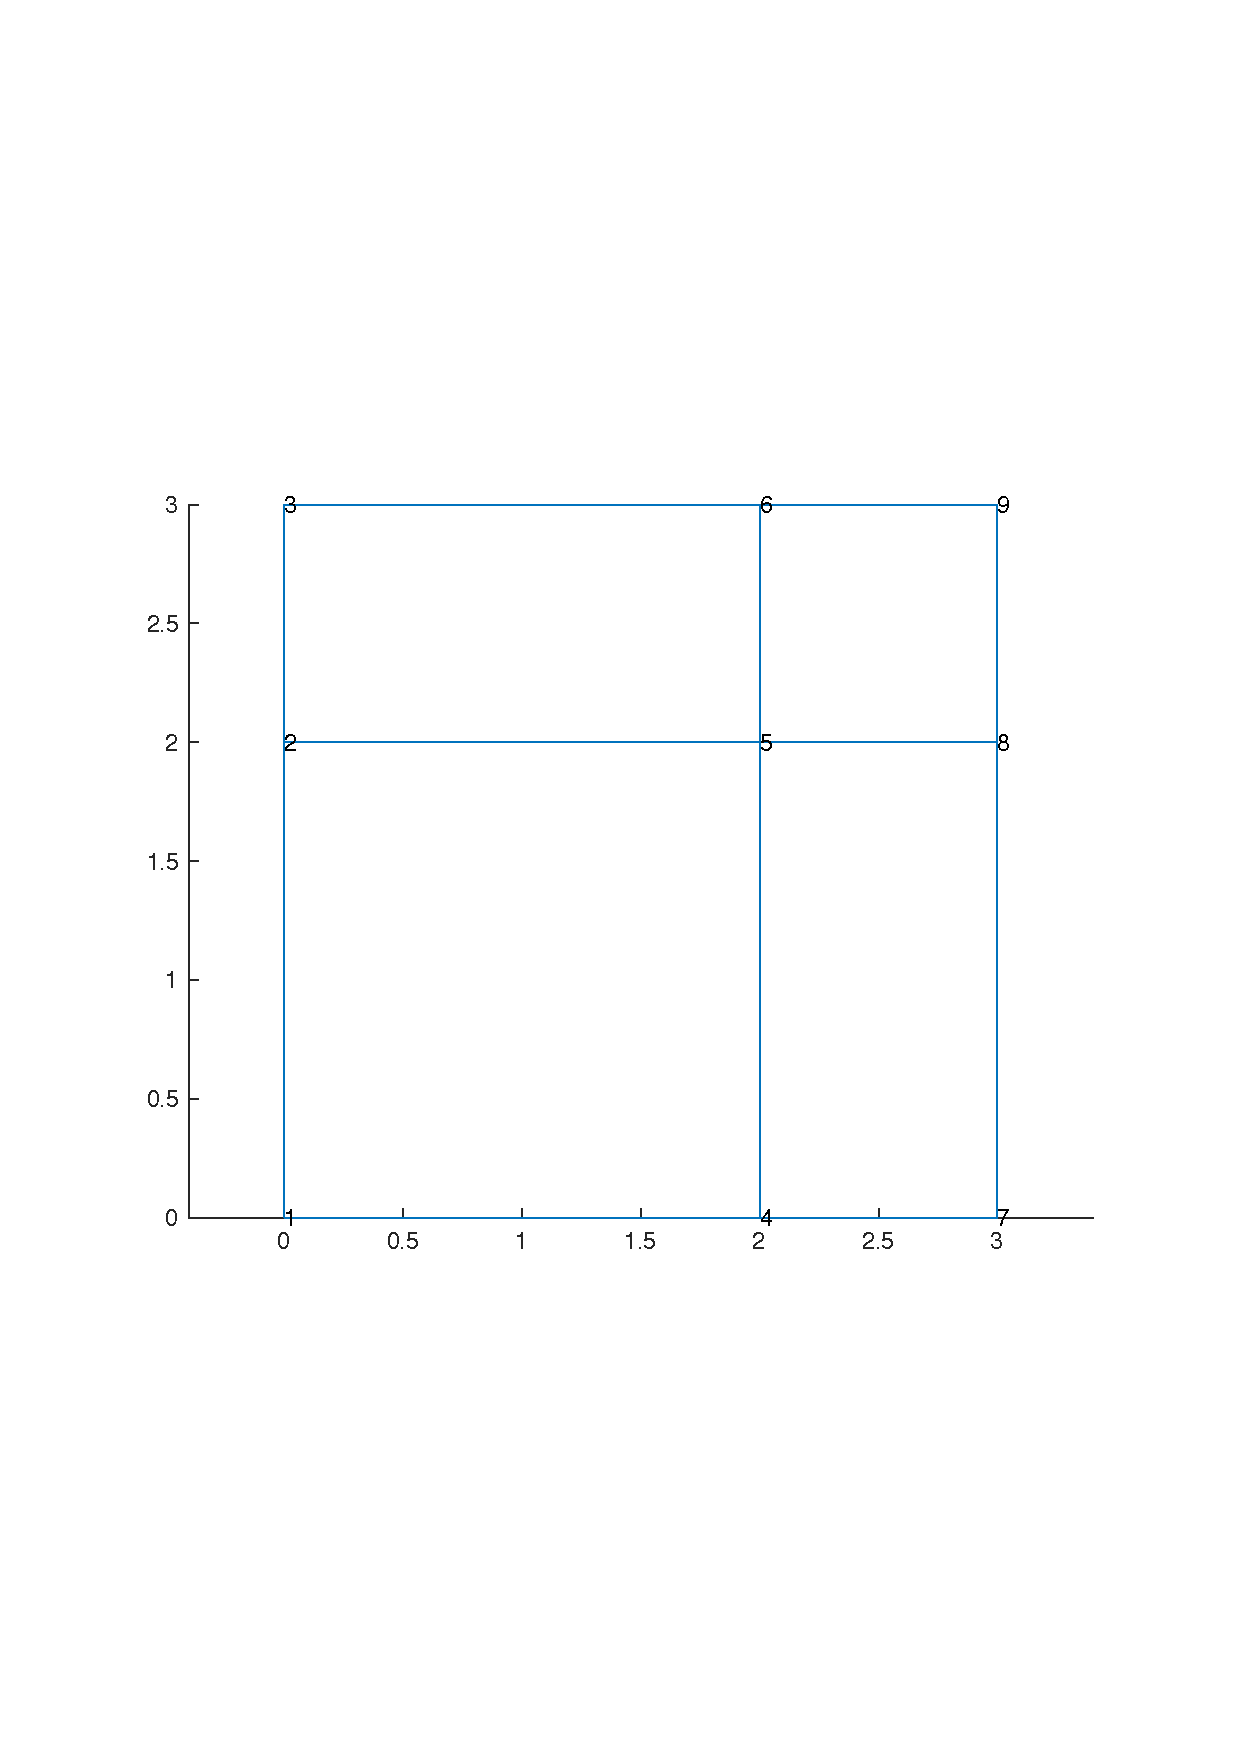
\includegraphics[width=0.65\linewidth]{patchtestxshell.pdf}  
	\caption{分块示意图} 
	\label{fig:mcmthesis-logo}
\end{figure}

在x方向单轴拉伸,使x方向应力大小为1Pa,应当满足线性场$x-disp=\frac{x}{3\times 10^7}$,$y-disp=\frac{y}{10^8}$($E=3\times10^7$,$\nu=0.3$)。从单轴拉伸的结果来看,很好地满足了构造的线性场。
\begin{figure}[h]
	\centering
	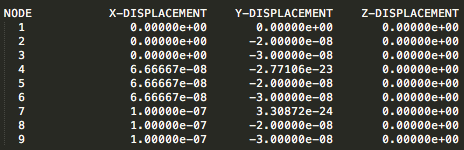
\includegraphics[width=0.65\linewidth]{shelltest.png}  
	\caption{单轴拉伸结果} 
	\label{fig:mcmthesis-logo}
\end{figure}


\section{连接单元}
针对两个点的约束,如果两个点位置在浮点数误差内一致,则直接在前处理中把两个点合并为一个点。然而,在前处理中处理约束时将两个点合并成一个点也有一定的复杂度。如果两个点的位置略有不同,则可以使用连接单元使两个点位移一致。考虑的方法是使用类似于罚函数的方法。建立的方法如下。
\begin{center}
$k\left[\begin{matrix}
I_6&-I_6\\
-I_6&I_6
\end{matrix}\right]\left[\begin{matrix}
d_{e1}\\d_{e2}
\end{matrix}\right]=\left[\begin{matrix}
f_{e1}\\f_{e2}
\end{matrix}\right]$
\end{center}
如此建立可以保证$f_{e1}+f_{e2}=0$,满足作用力与反作用力相等。$k(d_{e1}-d_{e2})=f_{e1}$。当k取一个数量级高于其余刚度阵的数量级的数时(可看作硬梁),则$d_{e1}-d_{e2}$趋于零,即可以视作两个节点被固接起来。综上,连接单元的刚度阵为
\begin{center}
$K=k\left[\begin{matrix}
I_6&-I_6\\
-I_6&I_6
\end{matrix}\right]$
\end{center}
使用了这样的连接单元后,在前处理时,就只需将两个约束的点之间加一个连接单元即可,k的大小随不同情况改变,需较别的刚度阵中元素高若干数量级。但也不能取得过大,否则会导致线性方程组条件数过大,其解由于截断误差不准确的问题。

%到此为止

\section{稀疏矩阵求解器}
我们选取了MKL库中的稀疏矩阵求解器PARDISO,PARDISO的基本原理是根据稀疏特性优化的LDLT分解算法,基于共享内存,同时具有多线程的并行性,是一种Left-looking Right-looking 结合的算法。
\subsection{稀疏矩阵的存储方式}
CSR是最流行和通用的格式,可为高性能架构中的结构化和非结构化稀疏矩阵提供出色的压缩比。 具有CSR格式的向量运算在CPU上实现时显示出良好的性能改进,并且所有算法(如BLAS,LAPACK和CUSparse)均支持此格式。 它使用三个1维数组,一个用于保存非零值,第二个用于保存每行非零值的数量,第三个用于保存非零值的列索引。此格式的大小主要取决于矩阵中的非零值的数量。 CSR较好的反映了矩阵的稀疏特性,并且受每行非零值的分布的影响。
\begin {equation} 
A_{\operatorname{man}}=\left[ \begin{array}{ccccc}{0} & {4} & {0} & {7} & {0} \\ {2} & {0} & {3} & {0} & {6} \\ {0} & {5} & {0} & {0} & {0} \\ {0} & {0} & {0} & {0} & {2} \\ {1} & {0} & {0} & {6} & {0}\end{array}\right]
 \end {equation}

\begin{equation} 
Data=\left[ \begin{array}{ccccccccc}{4} & {7} & {2} & {3} & {6} & {5} & {2} & {1} & {6}\end{array}\right]
 \end{equation}
\begin{equation} 
Column-indices=\left[ \begin{array}{lllllllll}{1} & {3} & {0} & {2} & {4} & {1} & {4} & {0} & {3}\end{array}\right]
 \end{equation}
\begin{equation} 
P t r=\left[ \begin{array}{llllll}{0} & {2} & {5} & {6} & {7} & {9}\end{array}\right]
 \end{equation}
CSR占据的存储空间为
\begin{equation} 
CSR_{\text {storage}}=2 \times N Z V+m+1
 \end{equation}
\subsection{稀疏矩阵的具体实现}
在原有的STAP++的LDLT求解器中适配的是Skyline格式的矩阵,对于Pardiso求解器,适配上述的CSR格式的求解器。CSR格式需要矩阵每一行的长度来分配内存,但在组装过程结束前并不能完全清楚每一行的长度,因此这设计到可变长度的存储非零元素的索引值,因此我们考虑到使用c++的<vector>容器来进行存储。\par
在最终使用vector之前我们对比了其他c++标准STL容器。他们具有一些共同优点,如接口简单,排序速度快,使用方便,内存分配科学。但在这一问题中,vector的特点适配的较好。vector是典型的序列容器,唯一可以和标准C兼容的stl容器,任意元素的读取、修改具有常数时间复杂度,在序列尾部进行插入、删除是常数时间复杂度,但在序列的头部插入、删除的时间复杂度是O(n),可以在任何位置插入新元素,有随机访问功能,插入删除操作需要考虑。排序的时间复杂度为O(NlogN)。
在程序的编写过程中,首先扫描全部元素,标记所有非零元的位置,为CSR求解器预先分配内存之后对存储的索引值进行排序,去掉重复的索引值,之后分配矩阵元素值的存储空间。
\subsection{PARDISO的参数调节}
根据系统的环境可以调节系统的并行线程数,在16核的系统上性能得到了大幅度的提升。同时打开OOC模式开关,MKL带有IC/OOC模式的开关,IC指的是IN-CORE的存储,OOC指的是out-of-core的存储方式,通俗的说IC模式将原本全部存储在内存中的文件中超出允许使用的内存上限的部分存储在硬盘中,因此解决了内存溢出的问题。OOC可以通过将矩阵因子保存在磁盘上的文件中来解决非常大的问题,与IC相比,这减小了对于内存的需求。通过MKL-PARDISO-OOC-MAX-CORE-SIZE这一变量规定OOC模式PARDISO能够使用的最大内存量。同时在工作目录下配置pardiso-ooc.cfg配置文件。
我们在本地电脑上对于第二个算例进行了OOC的尝试,配置文件为:\\
ooc-max-core-size got from config file=200 \\
ooc-max-swap-size got from config file=0 \\
ooc-keep-file     got from config file=1 \\
显示成功读取相关配置文件
最终结果如下:
\begin{table}[htbp]
  \centering
  \caption{PARDISO STATISTICS}

    \begin{tabular}{lcl}
   \multicolumn{3}{l}{TIMES} \\
 \hline
Time spent in calculations of symmetric matrix portrait (fulladj)&:& 0.115191 s \\
Time spent in reordering of the initial matrix (reorder)         &:& 0.394719 s \\
Time spent in symbolic factorization (symbfct)                  & :& 0.589268 s \\
Time spent in data preparations for factorization (parlist)     & :& 0.013076 s \\
Time spent in copying matrix to internal data structure (A to LU)&:& 0.000000 s \\
      Factorization: Time for writing to files & :& 0.000000 \\
      Factorization: Time for reading from files&:& 0.000000 \\
Time spent in factorization step (numfct)       &                 : &76.839788 s\\
      Solution:      Time for reading from files&: &0.505685 \\
Time spent in direct solver at solve step (solve)&                : &0.623790 s \\
Time spent in allocation of internal data structures (malloc)&    : &3.694331 s \\
Time spent in additional calculations                        &    : &0.765964 s \\
Total time spent                                             &    : &83.036128 s \\
\hline
    \end{tabular}%
  \label{tab:addlabel}%
\end{table}%
\begin{table}[H]
  \centering
  \caption{OUT OF CORE STATISTICS}

    \begin{tabular}{lcl}
\multicolumn{3}{c}{ ----------- Out of core time (in percent) --------------} \\
\hline
\multicolumn{3}{l}{Factorization step(100):} \\
      write to files & : & 0 \\
      read from files&:& 0 \\ 
      factorization - write and read&:& 100 \\
\hline 
\multicolumn{3}{l}{Solution step (100):} \\
      read from files&:& 81 \\
      solve - writeread&:& 19 \\
Total time (100):& & \\
      read from files&:& 0 \\
      total - write and read&: &100 \\
----------- Out of core Mb -------------- \\
Factorization step:& &\\
      write to files &:&      0.000 Mb\\
      read from files&: &     0.000 Mb\\
Solution step: & & \\
      read from files&:&    414.116 Mb \\
Total size of data transferred:&  & \\
      write and read    & :  &  414.116 Mb\\
\hline
    \end{tabular}%

  \label{tab:addlabel}%

\end{table}%

同时OOC模式解决了第四个算例的内存溢出的问题,通过将大部分的存储内容放在硬盘中,用时间换空间,具备了解决大型问题的能力。例如:{\color{red}原本第四个算例我们的计算会发生内存溢出的问题,无法求解,现在通过OOC模式,将矩阵存储在硬盘中,完成了第四个算例的求解,可能是全班唯一具备求解第四个算例的能力的小组},但很遗憾的是,我们现在第四个算例的求解时间大约在30分钟左右,超出了求解时间,这可以在未来通过进一步的优化来解决,但OOC模式使得求解超大型的问题具备了理论可能,当然对于矩阵的结构等可能也需要进一步的优化,以减轻对存储容量的需求。\par
另外在求解过程中,我们也通过任务管理器对程序运行所占据的内存和CPU使用率进行了监控,在实验室的测试平台中,第四个算例中,程序8线程运行,CPU基本一直接近满负荷运行,内存最高峰达到50GB,磁盘的读写速度最高达到了500MB/s级别的速度,在本地测试的第二个算例中,内存高峰达到了400MB,在IC模式下为700MB,但程序运行时磁盘的读写速度大幅度上升,达到了50MB/s,整体运行时间增长了4倍左右。\par
如果运行环境的磁盘的读写速度有较大幅度的提升,如更换为SSD固态硬盘,可能对程序整体的运行时间有较好的增益,同时可以进一步分配更大的可使用内存量,当前考虑到系统的安全,我们只分配了大约45G的可使用内存空间。这在未来都是可以考虑优化的方面。
%\section{5.1}
%Point D,N,I:vicinity of point load.Point B,F,J,M:re-entrant conrners.
%\section{5.2}

%For NbN method $f_1 = 3q/8$,$f_2 = (q/4+2q/3)*5/2 = 55q/24$,$f_3 = (2q/3+11q/12)*3/2=57q/24$,$f_4 = (q+11q/12)/2 = 23q/24$.\par
%For EbE method  $f_1 = 3q/4$,$f_2 = 3q/4 + 4q/3 = 25q/12$,$f_3 = (11q/12+4q/3)=27q/12$,$f_4 = 11q/12$.\par
%Both the lumping method gurantee the resultant force is correct.The EbE method also satisfy the equivalence principle i.e. gurantee the resultant torque.
%\section{5.3}
%\begin{figure}[H]
%\centering
%  \subfloat[a]{%
%    \includegraphics[width=.3\textwidth]{a.png}}\hfill
%  \subfloat[b]{%
%    \includegraphics[width=.3\textwidth]{b.png}}\hfill
%\subfloat[c]{%
%    \includegraphics[width=.3\textwidth]{c.png}}\\
%
%  \subfloat[d]{%
%    \includegraphics[width=.3\textwidth]{d.png}}\hfill
% \subfloat[e]{%
%    \includegraphics[width=.3\textwidth]{e.png}}\hfill
%\subfloat[f]{%
%    \includegraphics[width=.3\textwidth]{f.png}}\\
%  \caption{Symmetry and asymmetry lines and Boudary condition}\label{fig:2}
%\end{figure}
%For problem a,the vertical and horizontal diameter is symmetry and the D BCs is along the lines.\\
%For problem b,both the 45degree direction is the antisymmetry line and the D BCs is vertical to the lines.\\
%For problem c,the horizontal line is antisymmetry line and the D BC is vertical.\\
%For problem d,the vertical and horizontal line is symmetry line and D BCs is along the line.\\
%For problem d,the vertical line alone the concentrated load is symmetry line and D BC is along the line.\\
%For problem e,the vertical line placed in the middle of the loads is antisymmetry line and D BCs is horizontal.
%\chapter{Appendix}
%I'm truly sorry that the images is rather ugly because I don't have sufficient PS skills(or other drawing applicant). Sincere thanks to TA for enduring that!
%\chapter{Abaqus Python Scripts}
%For the given Loads,considering the capacity of computer,I chose the following test cases.
%% Table generated by Excel2LaTeX from sheet 'Sheet1'
%\begin{table}[htbp]
%  \centering
%  \caption{Value of $\varphi$ $\theta$}
%    \begin{tabular}{|l|rrrrrrrrrrrr|}
%\hline
%    $\varphi$   & -90   & -75   & -60   & -45   & -30   & -15   & 0     & 15    & 30    & 45    & 60    & 75 \\
%    $\theta$ & 0     & 30    & 60    & 90    &       &       &       &       &       &       &       &  \\
%\hline
%    \end{tabular}%
%  \label{tab:addlabel}%
%\end{table}%/////
%The Result of the models is shown below. The whole model's internal energy met its minimum in the following cases.
%% Table generated by Excel2LaTeX from sheet 'Sheet1'

%The optimal values are
%\begin{equation}
%\begin{cases}
%\varphi = -30,E=40594& \theta = 0 \\
%\varphi = 30,E=29151& \theta = 30 \\
%\varphi = 30,E=11177& \theta = 60 \\
%\varphi = 0,E=3543& \theta = 90 \\
%\end{cases}
%\end{equation}
%The optimal internal energy cases's stress nephogram is given below.
%\begin{figure}[H]
%\centering
%  \subfloat[$\theta = 0 ,\phi = -30$]{%
%    \includegraphics[width=.5\textwidth]{T0P-30.png}}\hfill
%  \subfloat[$\theta = 30 ,\phi = 30$]{%
%    \includegraphics[width=.5\textwidth]{T30P30.png}}\\
%  \subfloat[$\theta = 60 ,\phi = 30$]{%
%    \includegraphics[width=.5\textwidth]{T60P30.png}}\hfill
% \subfloat[$\theta = 90 ,\phi = 0$]{%
%    \includegraphics[width=.5\textwidth]{T90P0.png}}\\
%  \caption{Stress nephogram}\label{fig:2}
%\end{figure}
%%%============================================================================================================%%%
%%%=== 参考文献 ========%%%

\cleardoublepage
\end{document}



